\documentclass[aspectratio=169]{ctexbeamer}
\definecolor{urls}{RGB}{137, 180, 250}
\definecolor{link_text}{RGB}{245, 224, 220}
\hypersetup{
  colorlinks,
  linkcolor=, % This config controls the jumps inside the pdf
  urlcolor=urls,
}
\renewcommand{\UrlFont}{\ttfamily\scriptsize}

\usetheme{AnnArbor}
\usepackage[style=Mocha,accent=Rosewater]{beamercolorthemecatppuccin}

\usefonttheme{serif}
\usefonttheme{professionalfonts}

\usepackage[T1]{fontenc}
\setmainfont{LXGW WenKai}
% \setmainfont{Cascadia Code NF}
% \setsansfont{}
\setmonofont{Cascadia Code NF}
\usepackage{xeCJK}
\setCJKmainfont{LXGW WenKai}
% \setCJKmainfont{}
\setCJKmonofont{Cascadia Code NF}
\newcommand{\nerd}[1]{\texttt{#1}}
\setmonofont{Cascadia Code NF}[
  Contextuals=Alternate
]

\PassOptionsToPackage{hyphens}{url}
% \usepackage{ulem}
\usepackage{graphicx}
%\usepackage{wrapfig}
\usepackage{pifont} % Symbols used as itemize symbols
\usepackage{enumitem}
\setlist[itemize,1]{label={\small\color[RGB]{242, 205, 205}\ding{111}}}
\setlist[itemize,2]{label={\footnotesize\color[RGB]{242, 205, 205}\ding{111}}}
\usepackage{float}
\usepackage{booktabs}

\setbeamerfont{footnote}{size=\tiny}
\setbeamertemplate{footnote}{%
  \color[RGB]{108, 112, 134}%
  \insertfootnotetext%
}
\setlength{\footnotesep}{0.3\baselineskip}
\newcommand{\refnote}[1]{\footnotetext{#1}}

\usetheme{AnnArbor}

\usepackage{amsmath, amssymb, amsthm}
\usepackage{listings}
\lstdefinestyle{bash}{
  alsoletter=-,
  keywordstyle=[2]{\color[RGB]{243, 139, 168}},
  morekeywords=[2]{sudo},
  keywordstyle=[3]{\color[RGB]{166, 227, 161}},
  morekeywords=[3]{add-apt-repository, apt-get, apt},
  keywordstyle=[4]{\color[RGB]{250, 179, 135}},
  morekeywords=[4]{install},
}
\lstdefinestyle{lua}{
  alsoletter=-,
  keywordstyle=[2]{\color[RGB]{137, 180, 250}},
  morekeywords=[2]{name, priority, opts, config, dependencies, submodules, main, version, init, number, boolean},
  keywordstyle=[3]{\color[RGB]{180, 190, 254}},
  morekeywords=[3]{fun, setup},
  keywordstyle=[4]{\color[RGB]{250, 179, 135}},
  morekeywords=[4]{},
}
\lstdefinestyle{path}{
  alsoletter=~,
  basicstyle={\footnotesize\ttfamily\color[RGB]{147, 153, 178}\itshape},
}
\lstset{
  language={[5.1]lua},
  style=lua,
  basicstyle=\footnotesize\ttfamily,
  breaklines=true,
  showstringspaces=false,
  breakatwhitespace=true,
  keywordstyle=\color[RGB]{245, 169, 127},
  numberstyle={\ttfamily\color[RGB]{110, 115, 141}},
  commentstyle={\color[RGB]{147, 153, 178}\itshape},
  stringstyle={\color[RGB]{166, 218, 149}},
}
% NOTE: \lstinline{} command does not support background color
\lstdefinestyle{nvim}{
  alsoletter=:,
  keywordstyle=[3]{\color[RGB]{166, 227, 161}},
  morekeywords=[3]{:Tutor, :help}, % ChkTeX 26
}

\newcommand{\TODO}[1]{\textcolor{red}{TODO\@: #1} }

% \newcommand{\link}[3][]{\href{#3}{#2}\footnote[#1]{\url{#3}}}
\newcommand{\link}[3][]{\href{#3}{#2\textsuperscript{\nerd{}}}}



\title{Neovim从入门到出门}
\subtitle{第二节:界面美化(一)}
\author{Jacky-Lzx}
\date{\today}

\usepackage{tikz}
\titlegraphic {
  \begin{tikzpicture}[overlay,remember picture]
    \node at (-6, 4.5){
      
\includegraphics[height=1cm]{./Figures/Neovim_logo.png}
    };
    \node at (6, 4.5){
      
\includegraphics[height=1cm]{./Figures/Catppuccin_logo.png}
    };
  \end{tikzpicture}
}

\usepackage{makecell}

\begin{document}

\begin{frame}
  \titlepage
\end{frame}

\begin{frame}{大纲}
  \tableofcontents
\end{frame}
% Current section
\AtBeginSection[ ] {
  \begin{frame}{大纲}
    \tableofcontents[currentsection]
  \end{frame}
}

\section{Lazy.nvim插件配置介绍}
  \begin{frame}{Lazy.nvim插件配置介绍}

    在Lazy.nvim中,用一个table(\texttt{LazySpec})描述一个插件,一部分配置项见下表(完整的配置项请查阅\link{Lazy.nvim文档}{https://lazy.folke.io/spec}) % ChkTeX 19

    \begin{table}[H]
      \centering
      \small
      \begin{tabular}{ccp{8cm}}
        \toprule
        配置项          & 类型                                          & 介绍                          \\
        \midrule
        {[1]}        & \lstinline{string}    & \makecell[l]{插件的短链接                               \\例如\lstinline{"folke/noice.nvim"}所指的插件的网址为\\\lstinline{"github.com/folke/noice.nvim"}} \\ % ChkTex 18
        dependencies & \lstinline{LazySpec[]}                      & 依赖的插件,若有多个依赖插件,将其放入一个table中 \\
        priority     & \lstinline{number}                          & 插件加载的优先级,数值越大优先级越高          \\
        \bottomrule
      \end{tabular}
    \end{table}

  \end{frame}

  \begin{frame}{Lazy.nvim插件配置介绍}

    插件配置相关的配置项:

    \begin{table}[H]
      \centering
      \small
      \begin{tabular}{ccp{8cm}}
        \toprule
        配置项    & 类型                                & 介绍                                                                                                     \\
        \midrule
        main   & \lstinline{string}                & module的名字,一般情况下不需要配置,可被自动推导                                                                            \\
        init   & \lstinline{fun}                   & Neovim启动时执行的语句,无论插件有没有被加载                                                                              \\
        opts   & \lstinline{table}或\lstinline{fun} & 插件的配置表,用于\lstinline{setup(opts)}命令的调用                                                                  \\ % ChkTeX 36
        config & \lstinline{fun}或\lstinline{true}  & 插件加载时调用的函数,若\lstinline{opts}被设置或者\lstinline{config}为\lstinline{true},则自动调用插件的\lstinline{setup(opts)}方法 \\ % ChkTeX 36
        \bottomrule
      \end{tabular}
    \end{table}
  \end{frame}

  \begin{frame}{Lazy.nvim插件配置介绍}

    插件懒加载相关的配置项

    懒加载(Lazy loading):插件在Neovim启动时不加载,只有在满足一些条件时再加载

    \begin{table}[H]
      \centering
      \small
      \begin{tabular}{ccp{8cm}}
        \toprule
        配置项   & 类型                                                      & 介绍                         \\
        \midrule
        lazy  & \lstinline{boolean} & 如果为\lstinline{true},插件只有在需要的时候才加载                              \\
        event & \lstinline{string}...                                   & 插件懒加载的事件,在指定事件发生时加载插件      \\ % ChkTeX 11
        cmd   & \lstinline{string}...                                   & 在执行指定指令时加载插件               \\ % ChkTeX 11
        ft    & \lstinline{string}...                                   & 在打开指定类型的文件时加载插件            \\ % ChkTeX 11
        keys  & \lstinline{table}...                                    & 在按下指定的快捷键时加载插件(同时也定义这些快捷键) \\ % ChkTeX 11
        \bottomrule
      \end{tabular}
    \end{table}

  \end{frame}

  \begin{frame}[fragile]{Lazy.nvim插件配置介绍}
    举例

    \begin{lstlisting}
{
  'romgrk/barbar.nvim',
  version = '^1.0.0', -- optional: only update when a new 1.x version is released
  dependencies = {
    'lewis6991/gitsigns.nvim',
    'nvim-tree/nvim-web-devicons',
  },
  init = function() vim.g.barbar_auto_setup = false end,
  opts = {}, -- equivalent to the following
  -- config = function()
  --   require("barbar.nvim").setup({}) -- "barbar.nvim" is auto deduced by Lazy.nvim. If `main` property is set, use the content of `main` instead
  -- end
},
    \end{lstlisting}
  \end{frame}

\section{界面美化}

  \subsection{界面布局}
    \begin{frame}{界面布局 - 以VS Code为例}
      \begin{figure}[H]
        \centering
        
\includegraphics[width=0.75\linewidth]{./Figures/Vscode_interface.jpg}
      \end{figure}
    \end{frame}

    \begin{frame}{界面布局 - 以VS Code为例}

      \begin{columns}
        \begin{column}{0.25\linewidth}
          \begin{itemize}
            \item 为了更好地进行开发,我们需要:% ChkTeX 19
              \begin{enumerate}[label=\arabic*.]
                \item 状态栏
                \item 标签栏
                \item 文件列表
                \item 代码诊断
                \item 代码大纲
                \item 内置终端
              \end{enumerate}
            \item 本节我们实现前三个组件的配置
          \end{itemize}
        \end{column}

        \begin{column}{0.75\linewidth}
          \begin{figure}[H]
            \centering
            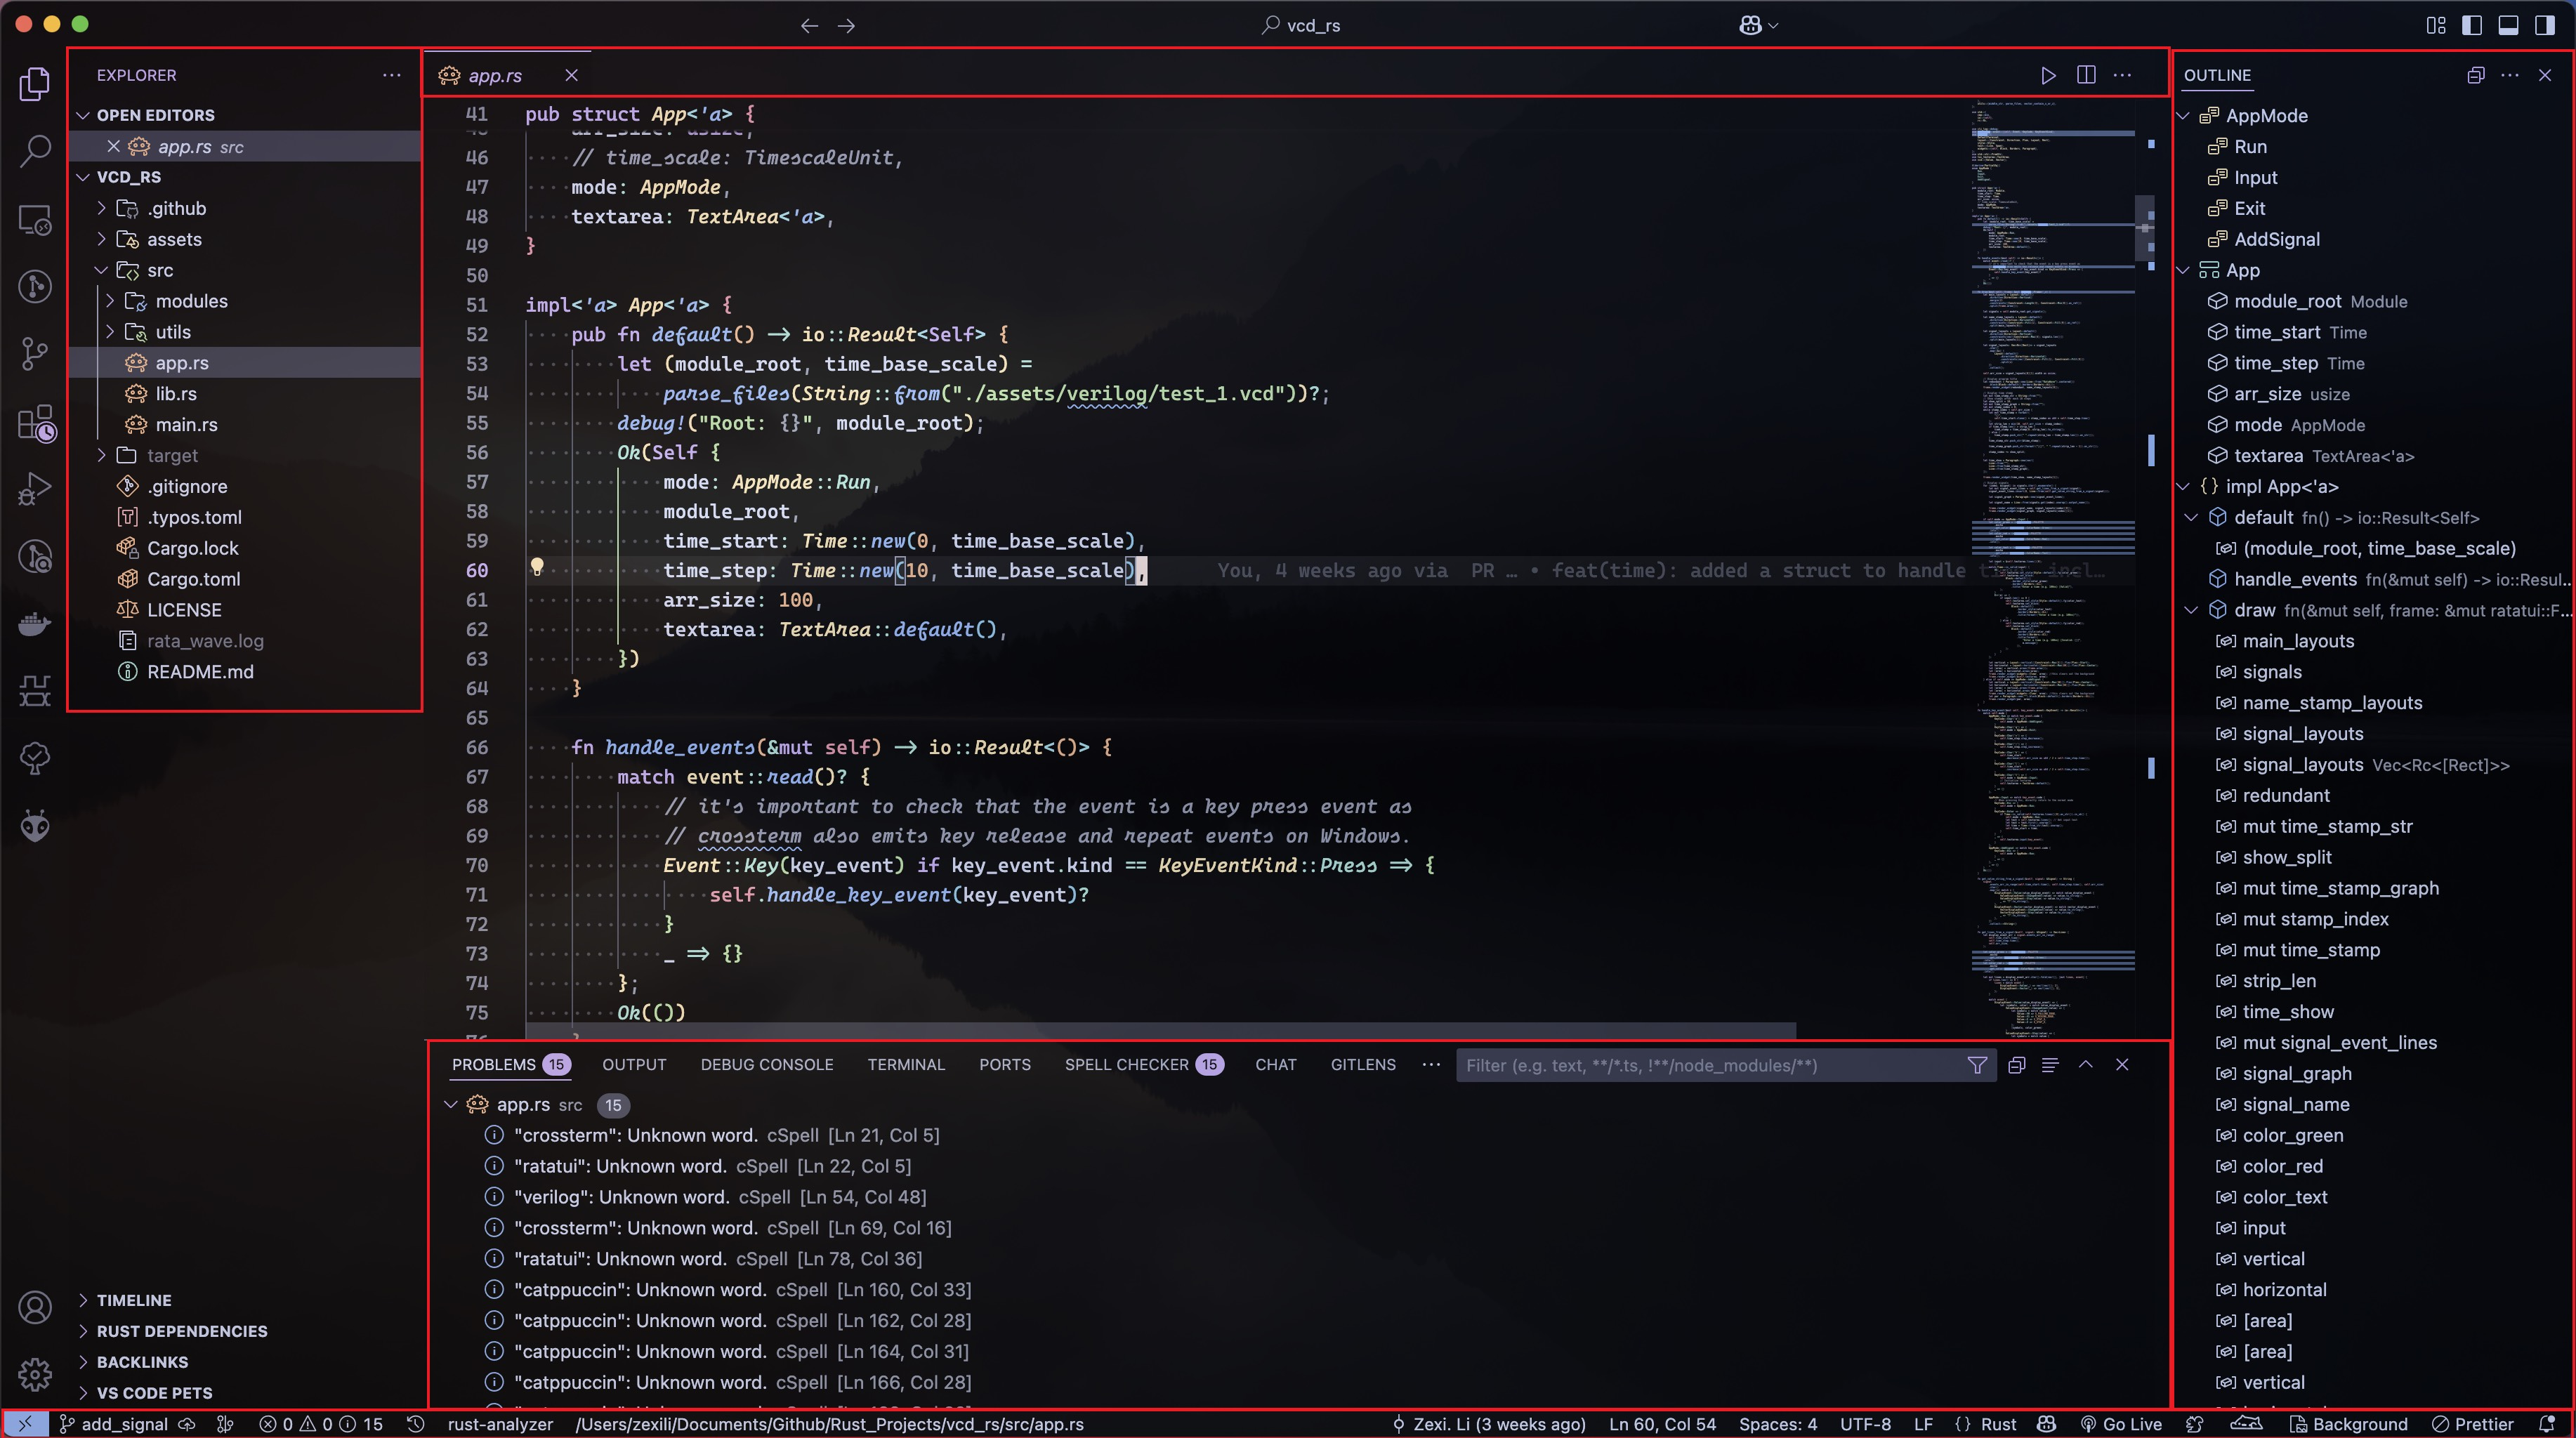
\includegraphics[width=0.9\linewidth]{./Figures/Vscode_interface_annotated.jpg}
          \end{figure}
        \end{column}
      \end{columns}

    \end{frame}

  \subsection{配色方案}
    \begin{frame}{配色方案(主题)}
      \link{Catppuccin}{https://catppuccin.com/} 
\includegraphics[height=10pt]{./Figures/Catppuccin_logo.png}
      \begin{columns}
        \begin{column}{0.45\linewidth}
          \begin{figure}[H]
            \centering
            
\includegraphics[width=\linewidth]{./Figures/Catppuccin.jpg}
          \end{figure}
        \end{column}

        \begin{column}{0.55\linewidth}
          \begin{figure}[H]
            \centering
            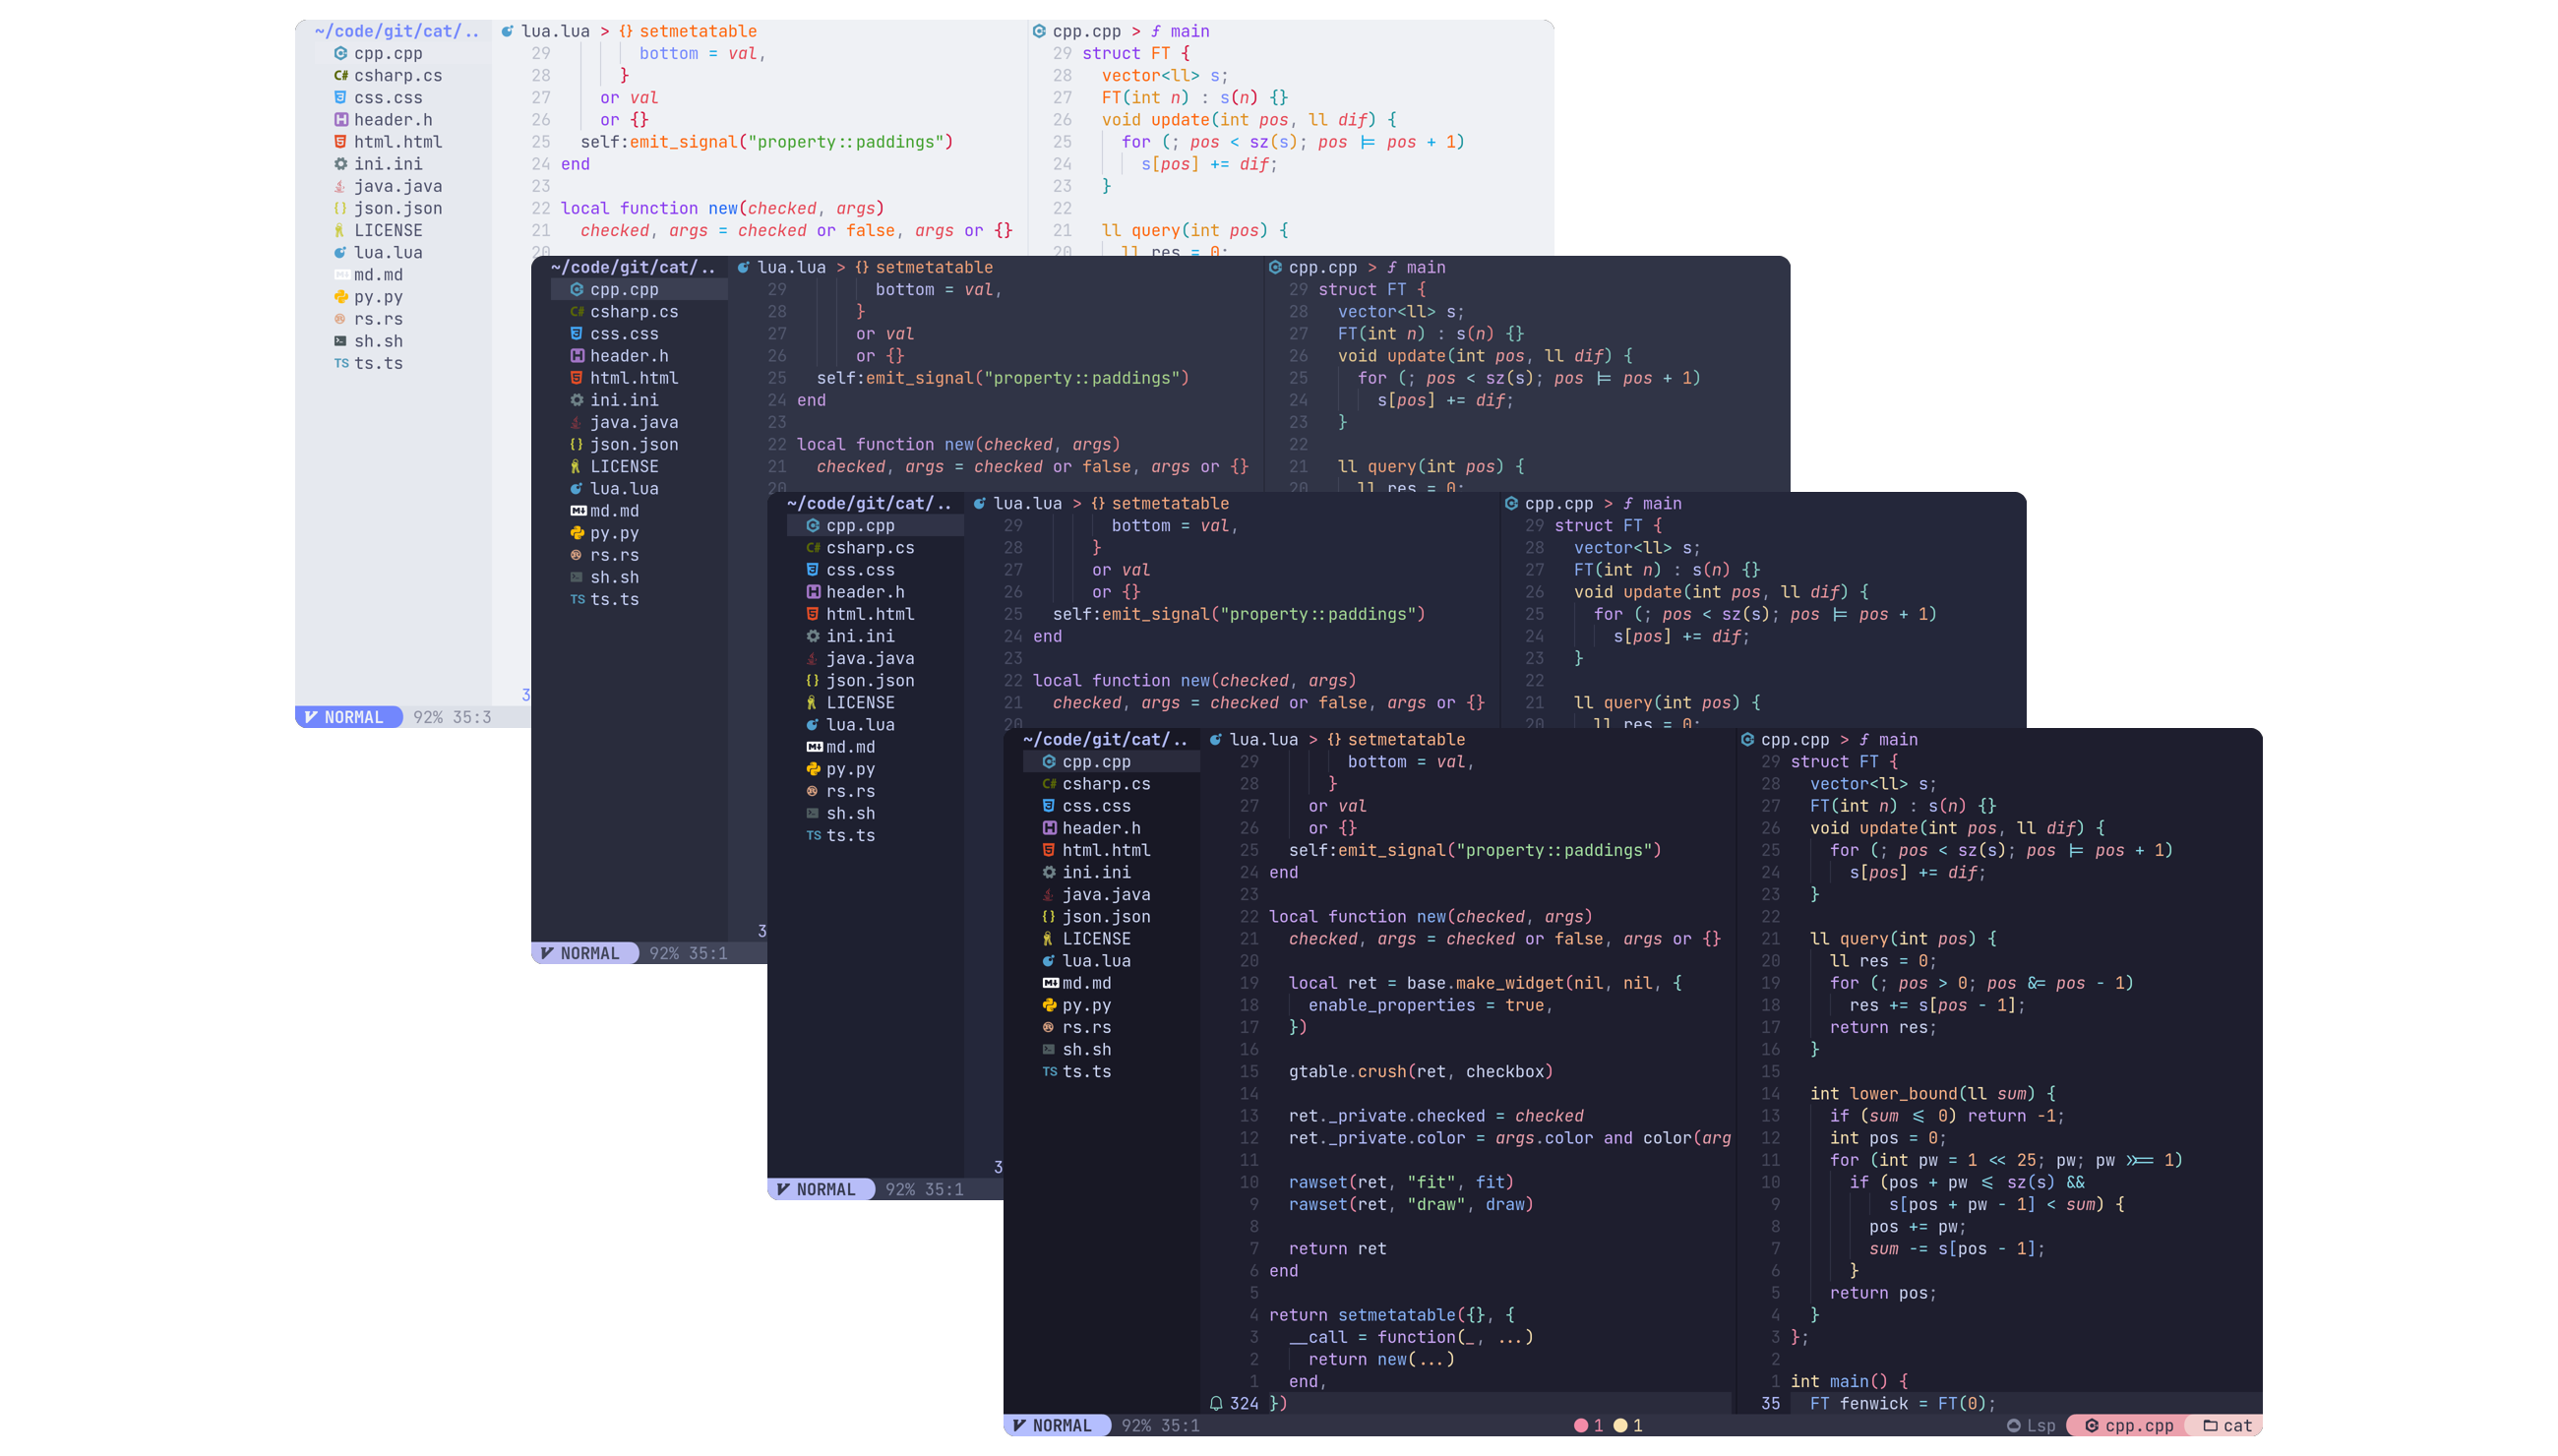
\includegraphics[width=\linewidth]{./Figures/Catppuccin_demo.png}
          \end{figure}
        \end{column}
      \end{columns}

      \refnote{图片:}
      \refnote{https://catppuccin.com/}
      \refnote{https://github.com/catppuccin/nvim}
    \end{frame}

\section{插件安装}

  \subsection{配色方案:catppuccin/nvim}
    \begin{frame}[fragile]{catppuccin/nvim}
      \link{catppuccin/nvim}{https://github.com/catppuccin/nvim}:Catppuccin配色方案的Neovim插件

      \begin{columns}
        \begin{column}{0.4\linewidth}
          \begin{lstlisting}[basicstyle=\tiny\ttfamily]
-- ~/.config/nvim/lua/plugins/colorscheme.lua

{
  "catppuccin/nvim",
  name = "catppuccin",
  priority = 1000,
  opts = {},
  config = function(_, opts)
    require("catppuccin").setup(opts)
    vim.cmd.colorscheme("catppuccin")
  end
}
      \end{lstlisting}
        \end{column}

        \begin{column}{0.6\linewidth}
          \begin{figure}[H]
            \centering
            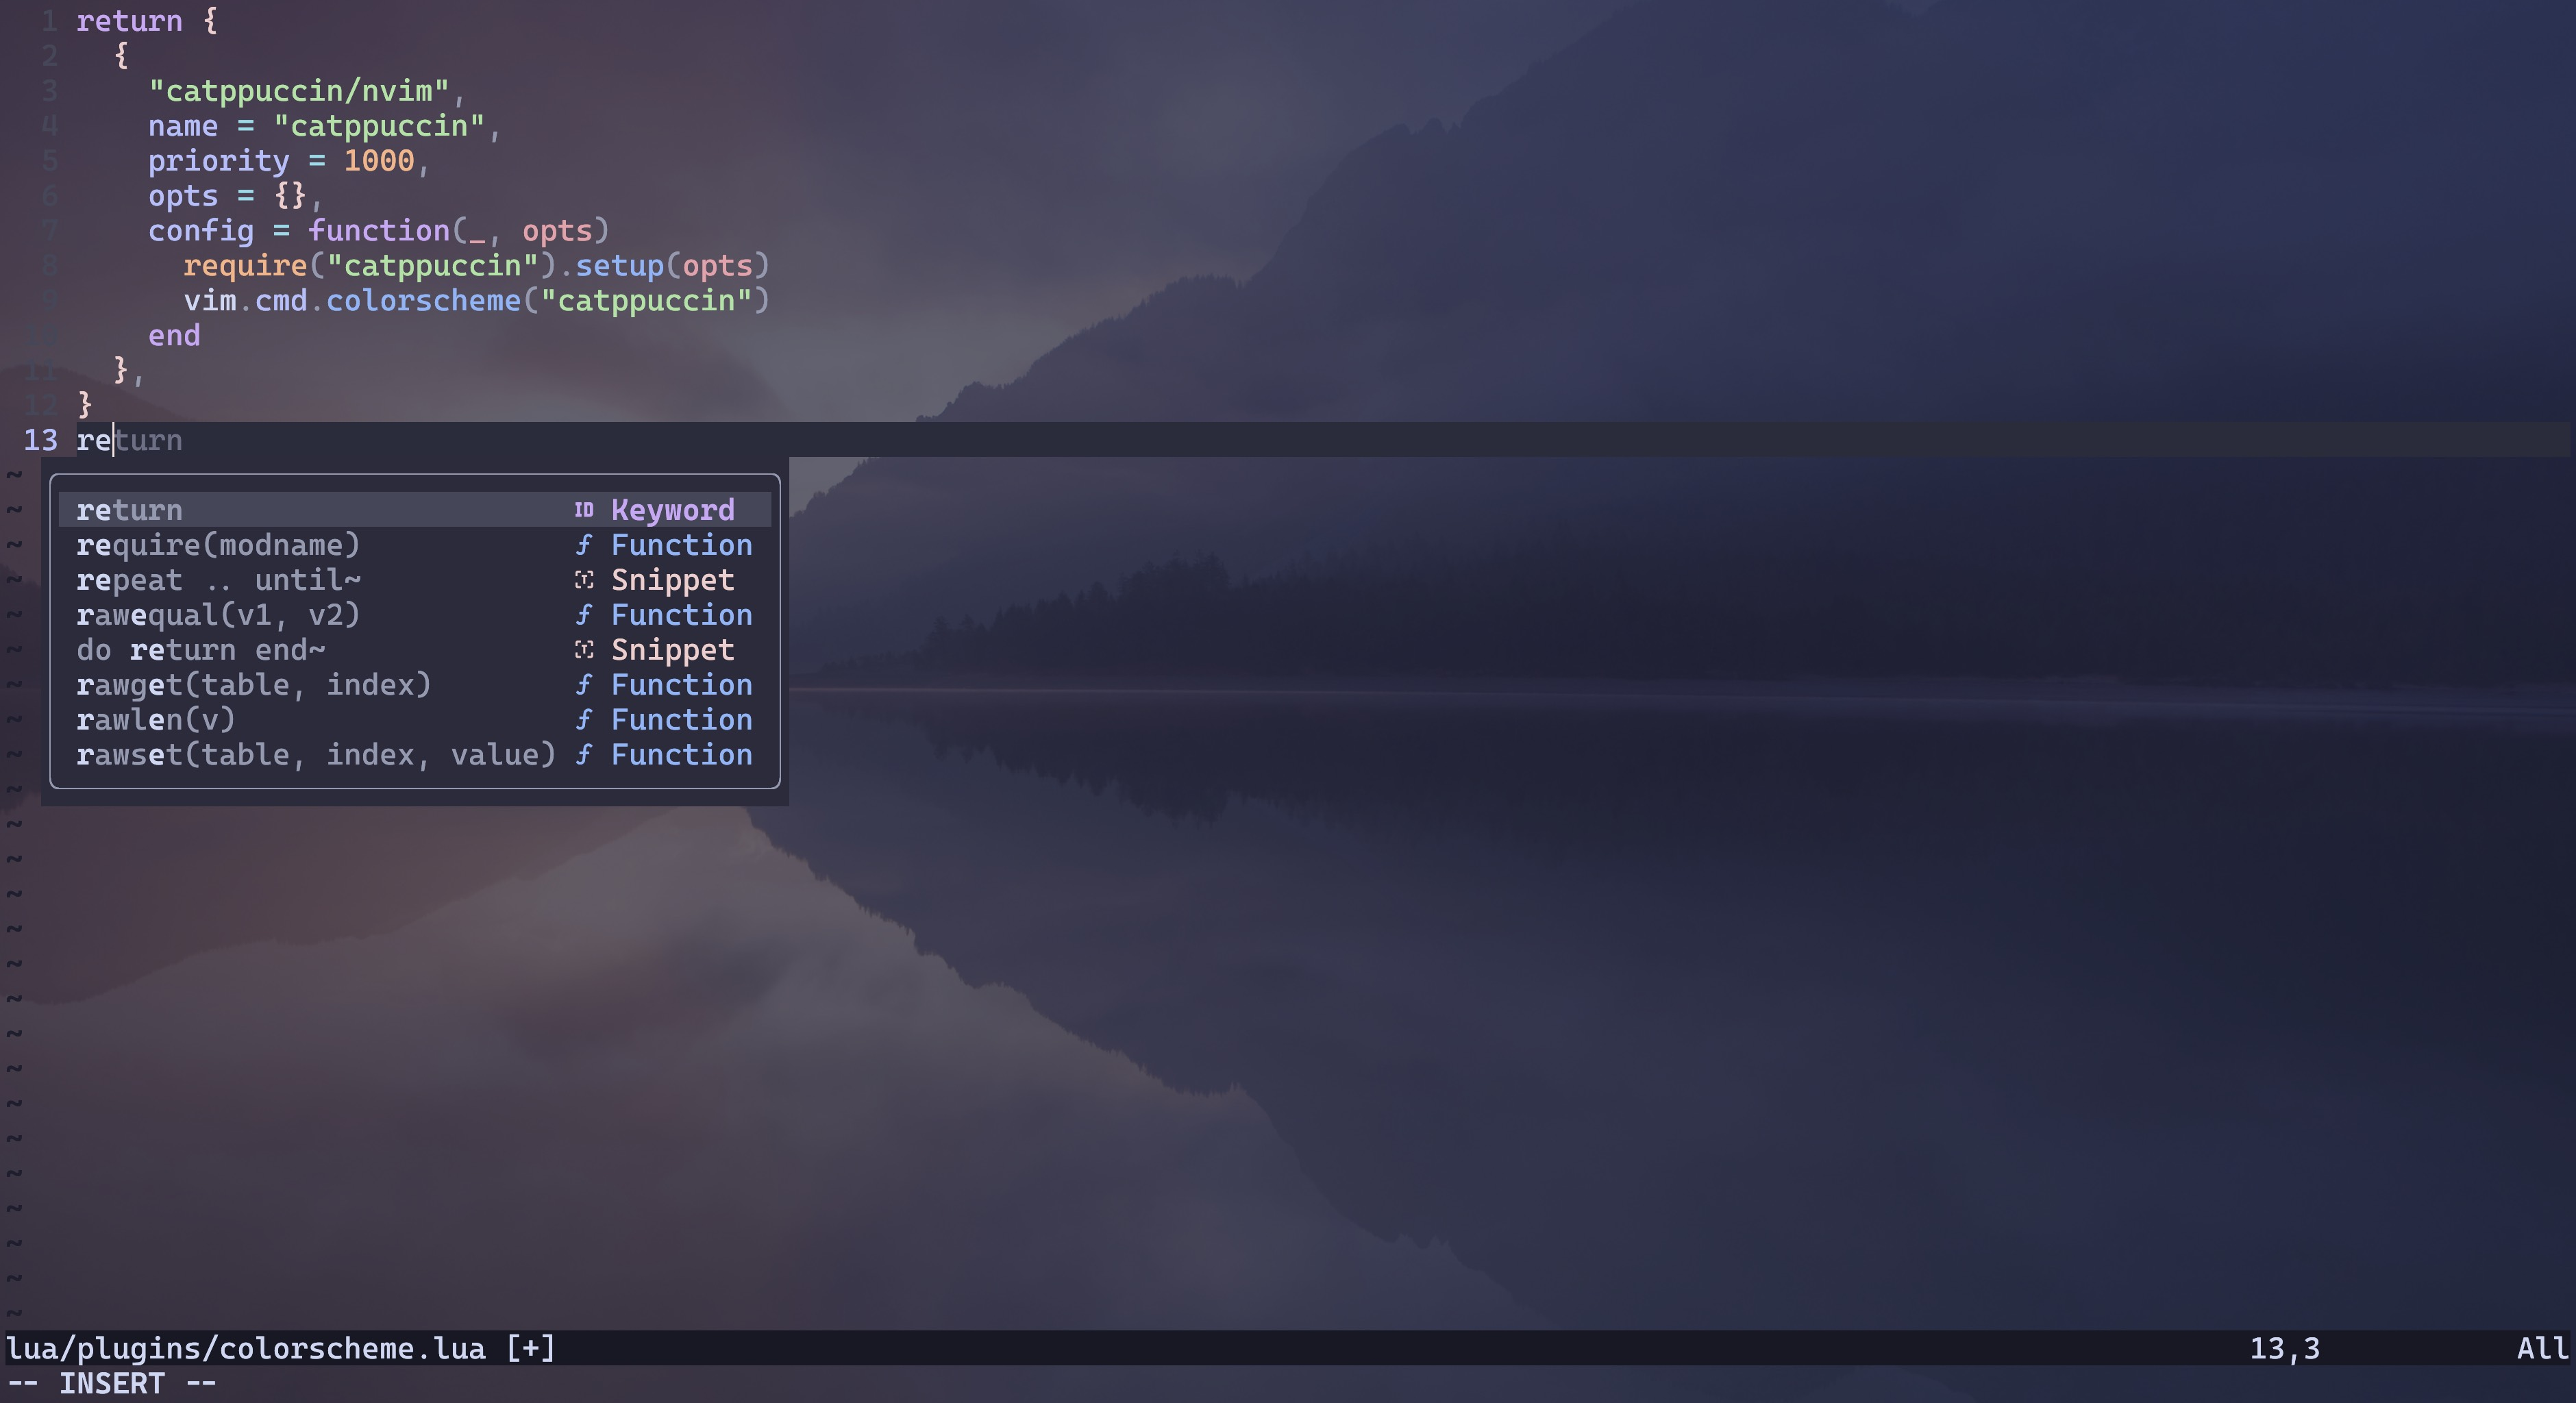
\includegraphics[width=\linewidth]{./Figures/Colorscheme_Finish.jpg}
            \caption{安装后的效果}%
          \end{figure}
        \end{column}
      \end{columns}

    \end{frame}

  \subsection{状态栏:lualine.nvim}
    \begin{frame}[fragile]{lualine.nvim}
      \link{lualine.nvim}{https://github.com/nvim-lualine/lualine.nvim}:Neovim状态栏

      \begin{columns}
        \begin{column}{0.4\linewidth}
          \begin{lstlisting}[basicstyle=\tiny\ttfamily]
-- ~/.config/nvim/lua/plugins/ui.lua

{
  'nvim-lualine/lualine.nvim',
  dependencies = {
    'nvim-tree/nvim-web-devicons'
  },
  opts = {}
}
          \end{lstlisting}
        \end{column}

        \begin{column}{0.6\linewidth}
          \begin{figure}[H]
            \centering
            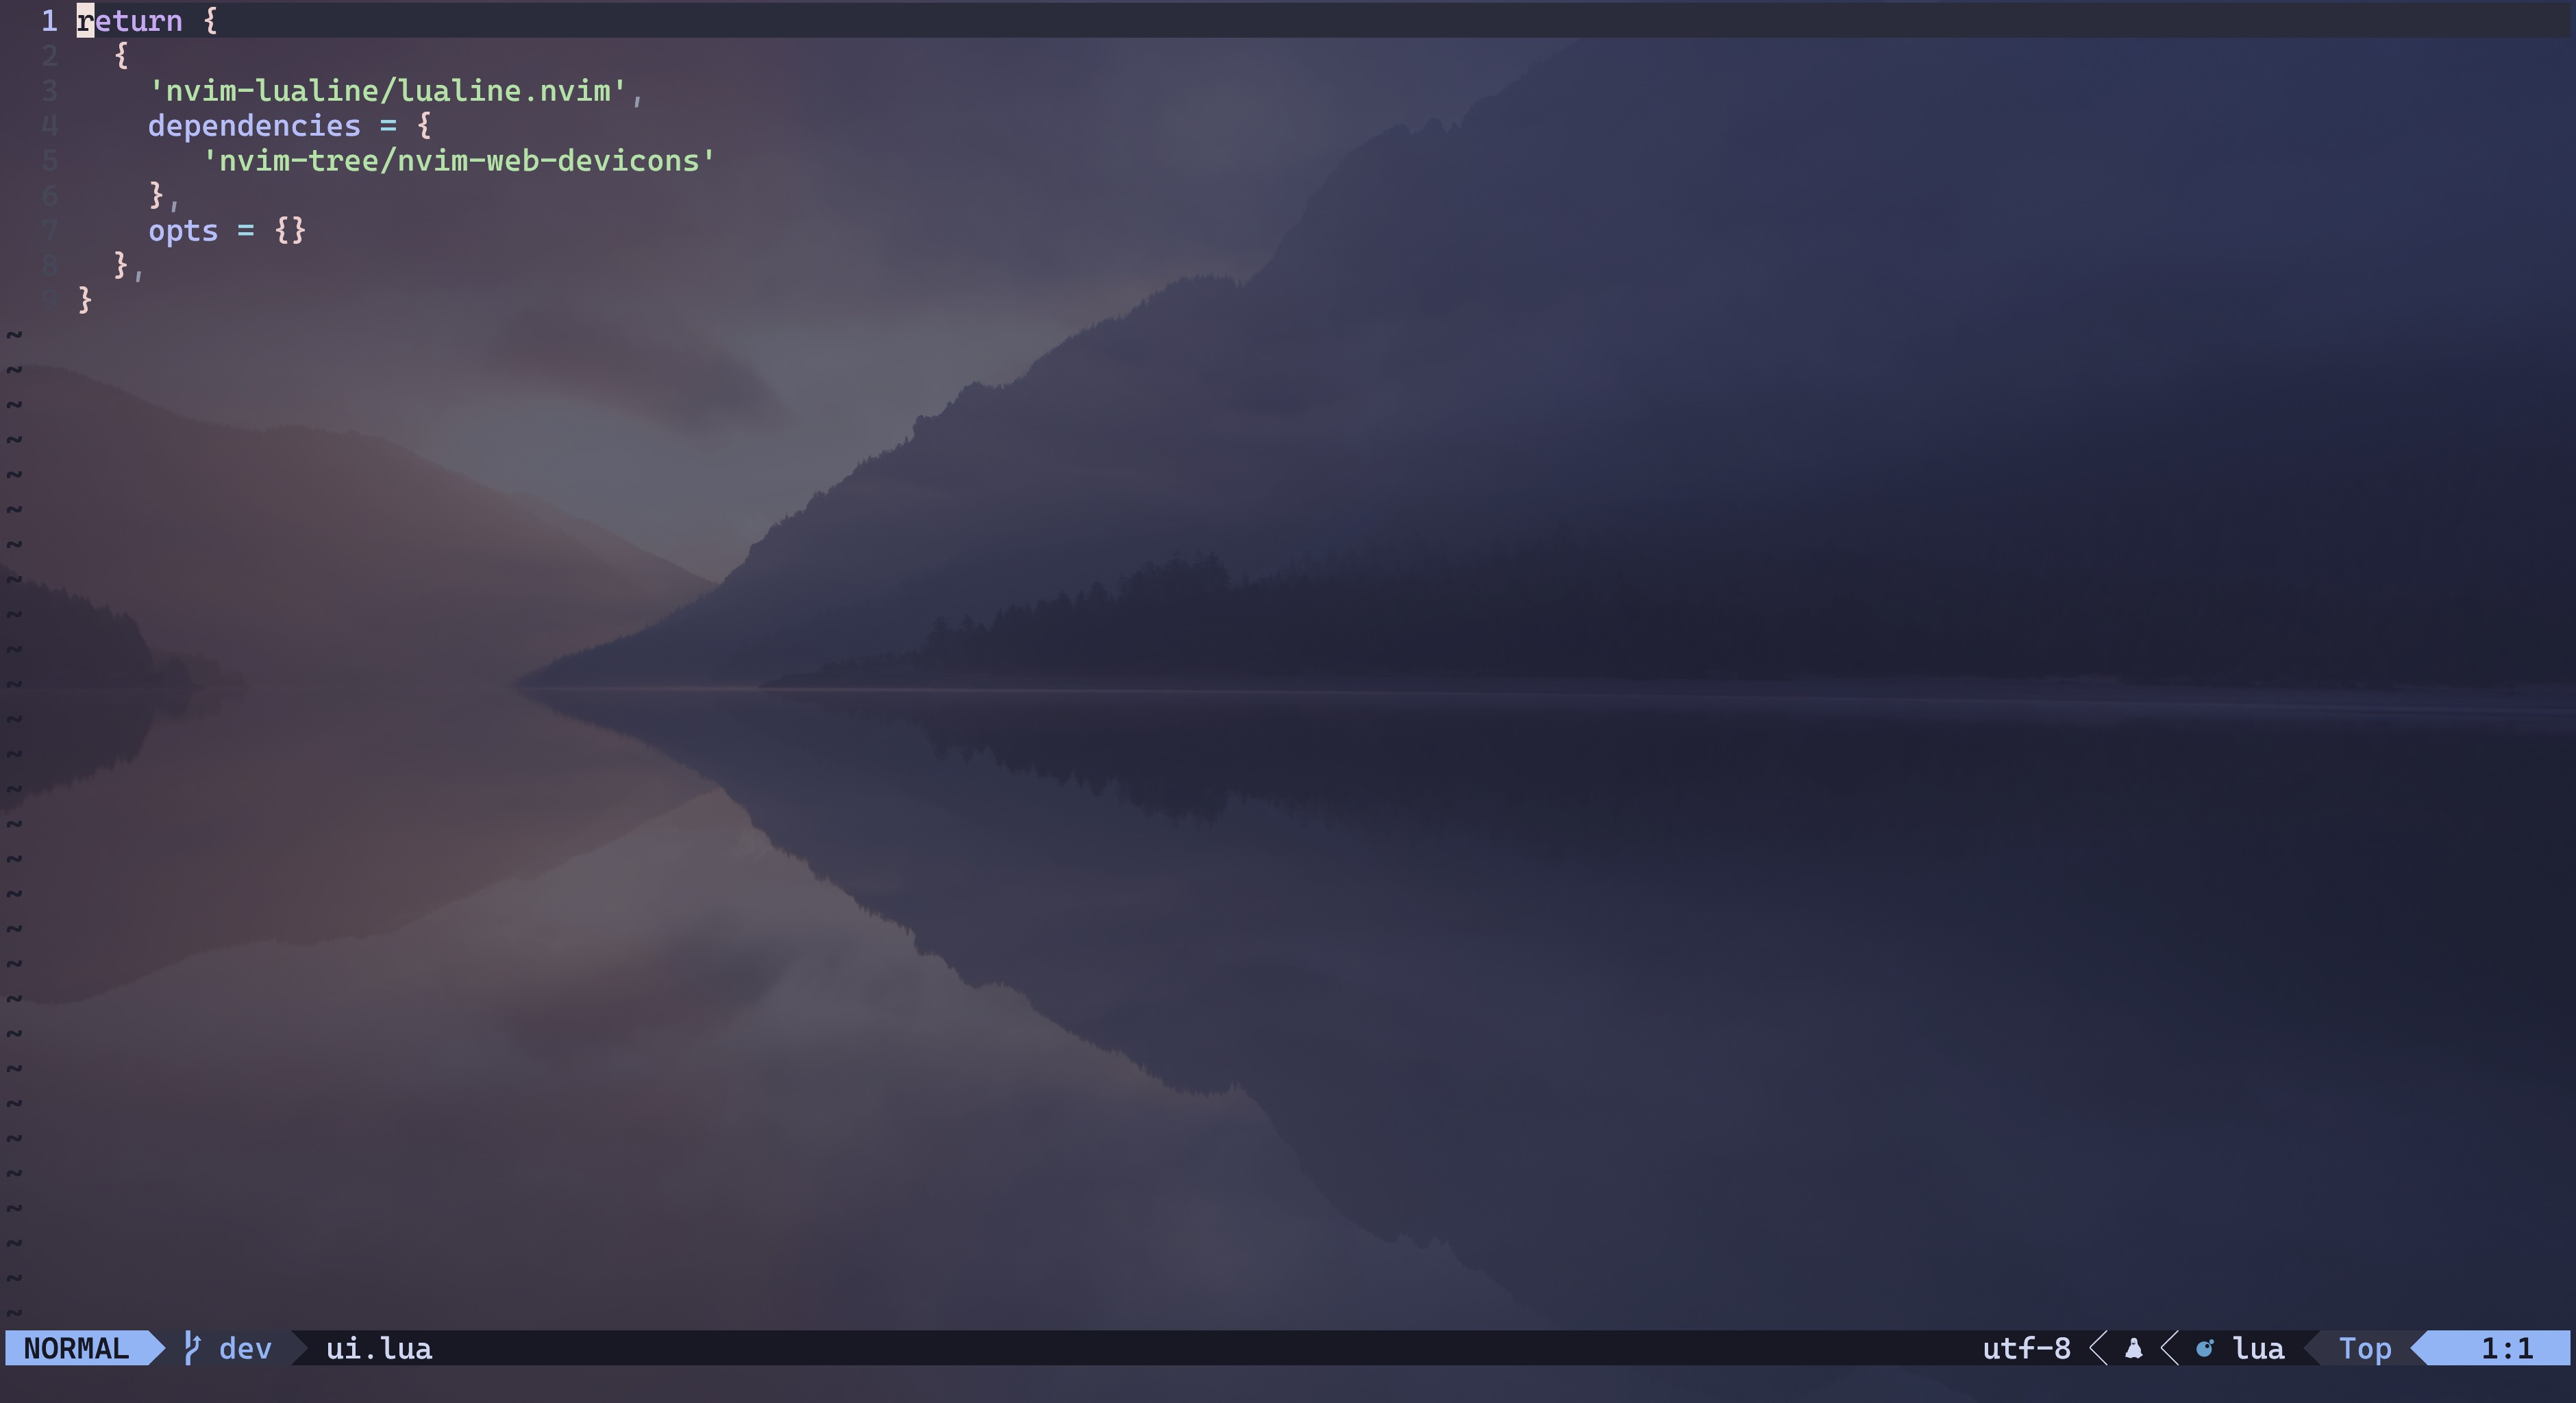
\includegraphics[width=\linewidth]{./Figures/Lualine_Finish.jpg}
            \caption{安装后的效果}%
          \end{figure}

        \end{column}
      \end{columns}

    \end{frame}

  \subsection{标签栏:barbar.nvim}
    \begin{frame}[fragile]{barbar.nvim}

      \link{barbar.nvim}{https://github.com/romgrk/barbar.nvim}:Neovim标签栏

      \begin{columns}
        \begin{column}{0.4\linewidth}
          \begin{lstlisting}[basicstyle=\tiny\ttfamily]
-- ~/.config/nvim/lua/plugins/ui.lua

{
  'romgrk/barbar.nvim',
  version = '^1.0.0', -- optional: only update when a new 1.x version is released
  dependencies = {
    'lewis6991/gitsigns.nvim',
    'nvim-tree/nvim-web-devicons',
  },
  init = function()
    vim.g.barbar_auto_setup = false
  end,
  opts = {},
}
          \end{lstlisting}
        \end{column}

        \begin{column}{0.6\linewidth}

          \begin{figure}[H]
            \centering
            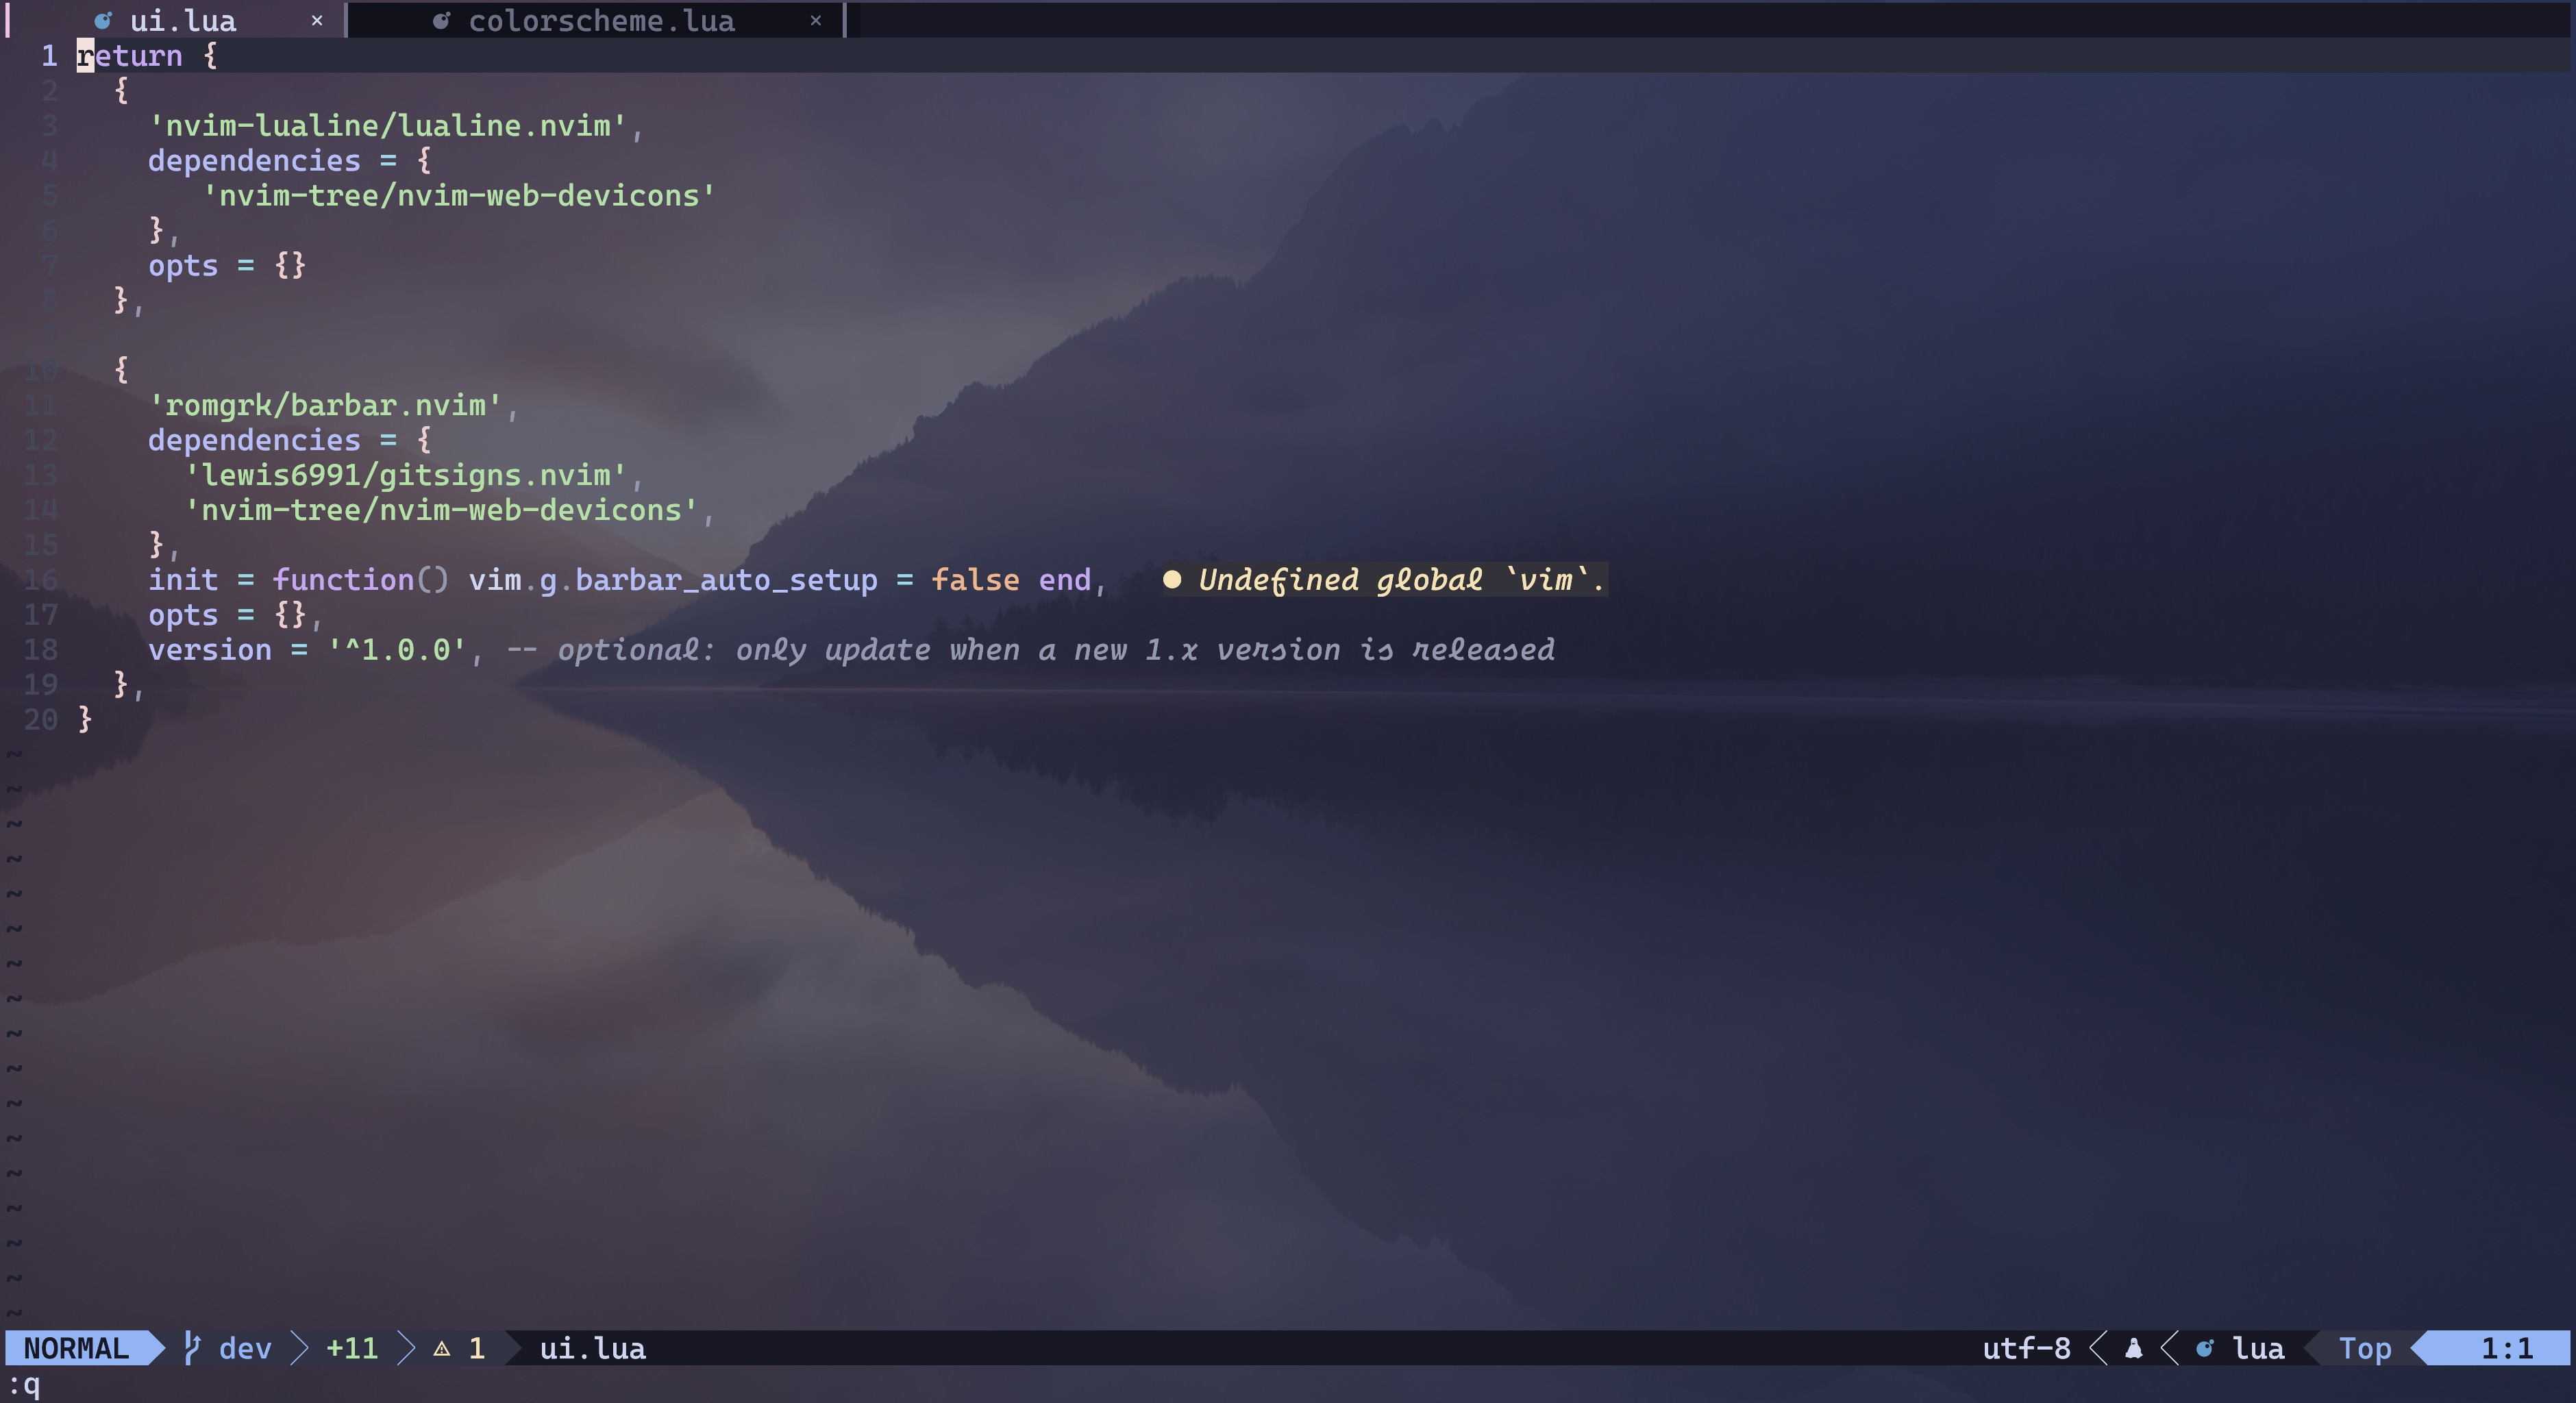
\includegraphics[width=\linewidth]{./Figures/Barbar_Finish.jpg}
            \caption{安装后的效果}%
          \end{figure}

        \end{column}
      \end{columns}

    \end{frame}

  \subsection{文件列表:nvim-tree.lua}
    \begin{frame}[fragile]{nvim-tree.lua}

      \link{nvim-tree.lua}{https://github.com/nvim-tree/nvim-tree.lua}:Neovim文件列表

      \begin{columns}
        \begin{column}{0.4\linewidth}
          \begin{lstlisting}[basicstyle=\tiny\ttfamily]
-- ~/.config/nvim/init.lua

-- disable netrw at the very start of your init.lua
vim.g.loaded_netrw = 1
vim.g.loaded_netrwPlugin = 1

-- ~/.config/nvim/lua/plugins/ui.lua

{
  "nvim-tree/nvim-tree.lua",
  version = "*",
  dependencies = {
    "nvim-tree/nvim-web-devicons",
  },
  opts = {}
}
          \end{lstlisting}
        \end{column}

        \begin{column}{0.6\linewidth}

          \begin{figure}[H]
            \centering
            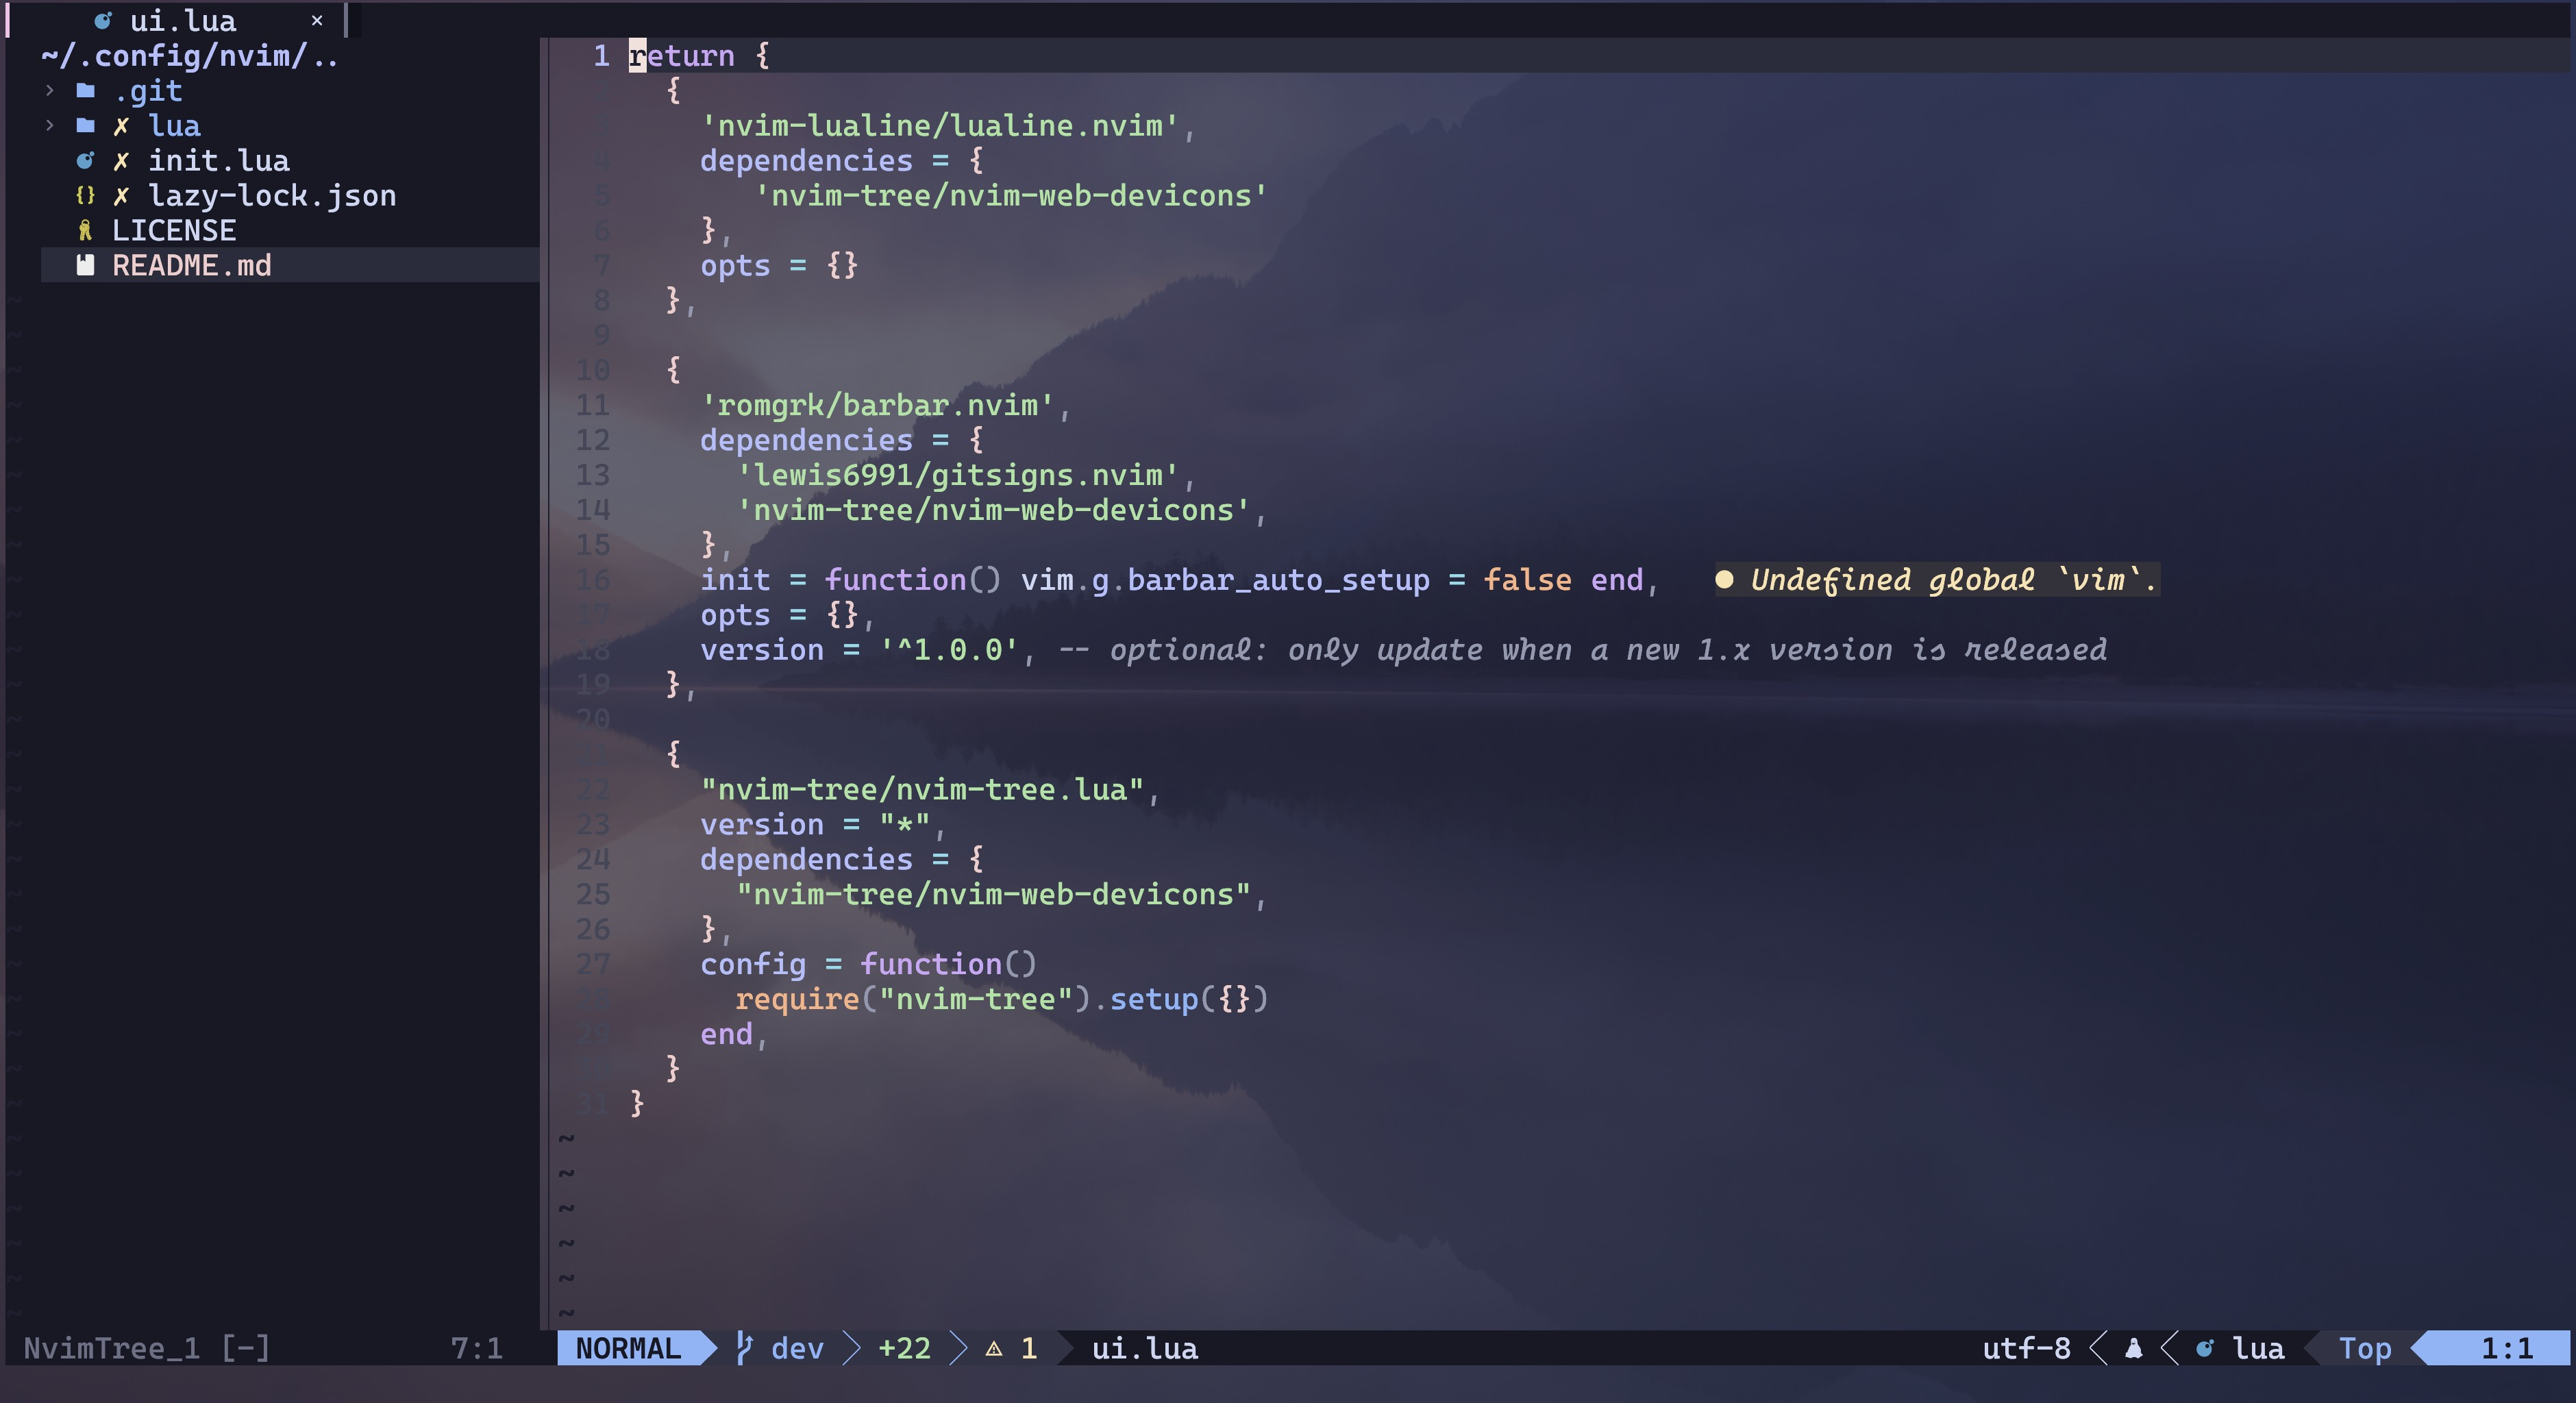
\includegraphics[width=\linewidth]{./Figures/NvimTree_Finish.jpg}
            \caption{安装后的效果}%
          \end{figure}

        \end{column}
      \end{columns}

    \end{frame}

  \subsection{多彩括号:rainbow-delimiters.nvim}
    \begin{frame}[fragile]{rainbow-delimiters.nvim}

      \link{rainbow-delimiters.nvim}{https://github.com/HiPhish/rainbow-delimiters.nvim}:不同深度的括号显示不同的颜色

      \begin{columns}
        \begin{column}{0.4\linewidth}
          \begin{lstlisting}[basicstyle=\tiny\ttfamily]
-- ~/.config/nvim/lua/plugins/ui.lua

{
  "HiPhish/rainbow-delimiters.nvim",
  submodules = false,
  main = "rainbow-delimiters.setup",
  opts = {}
}
          \end{lstlisting}
        \end{column}

        \begin{column}{0.6\linewidth}

          \begin{figure}[H]
            \centering
            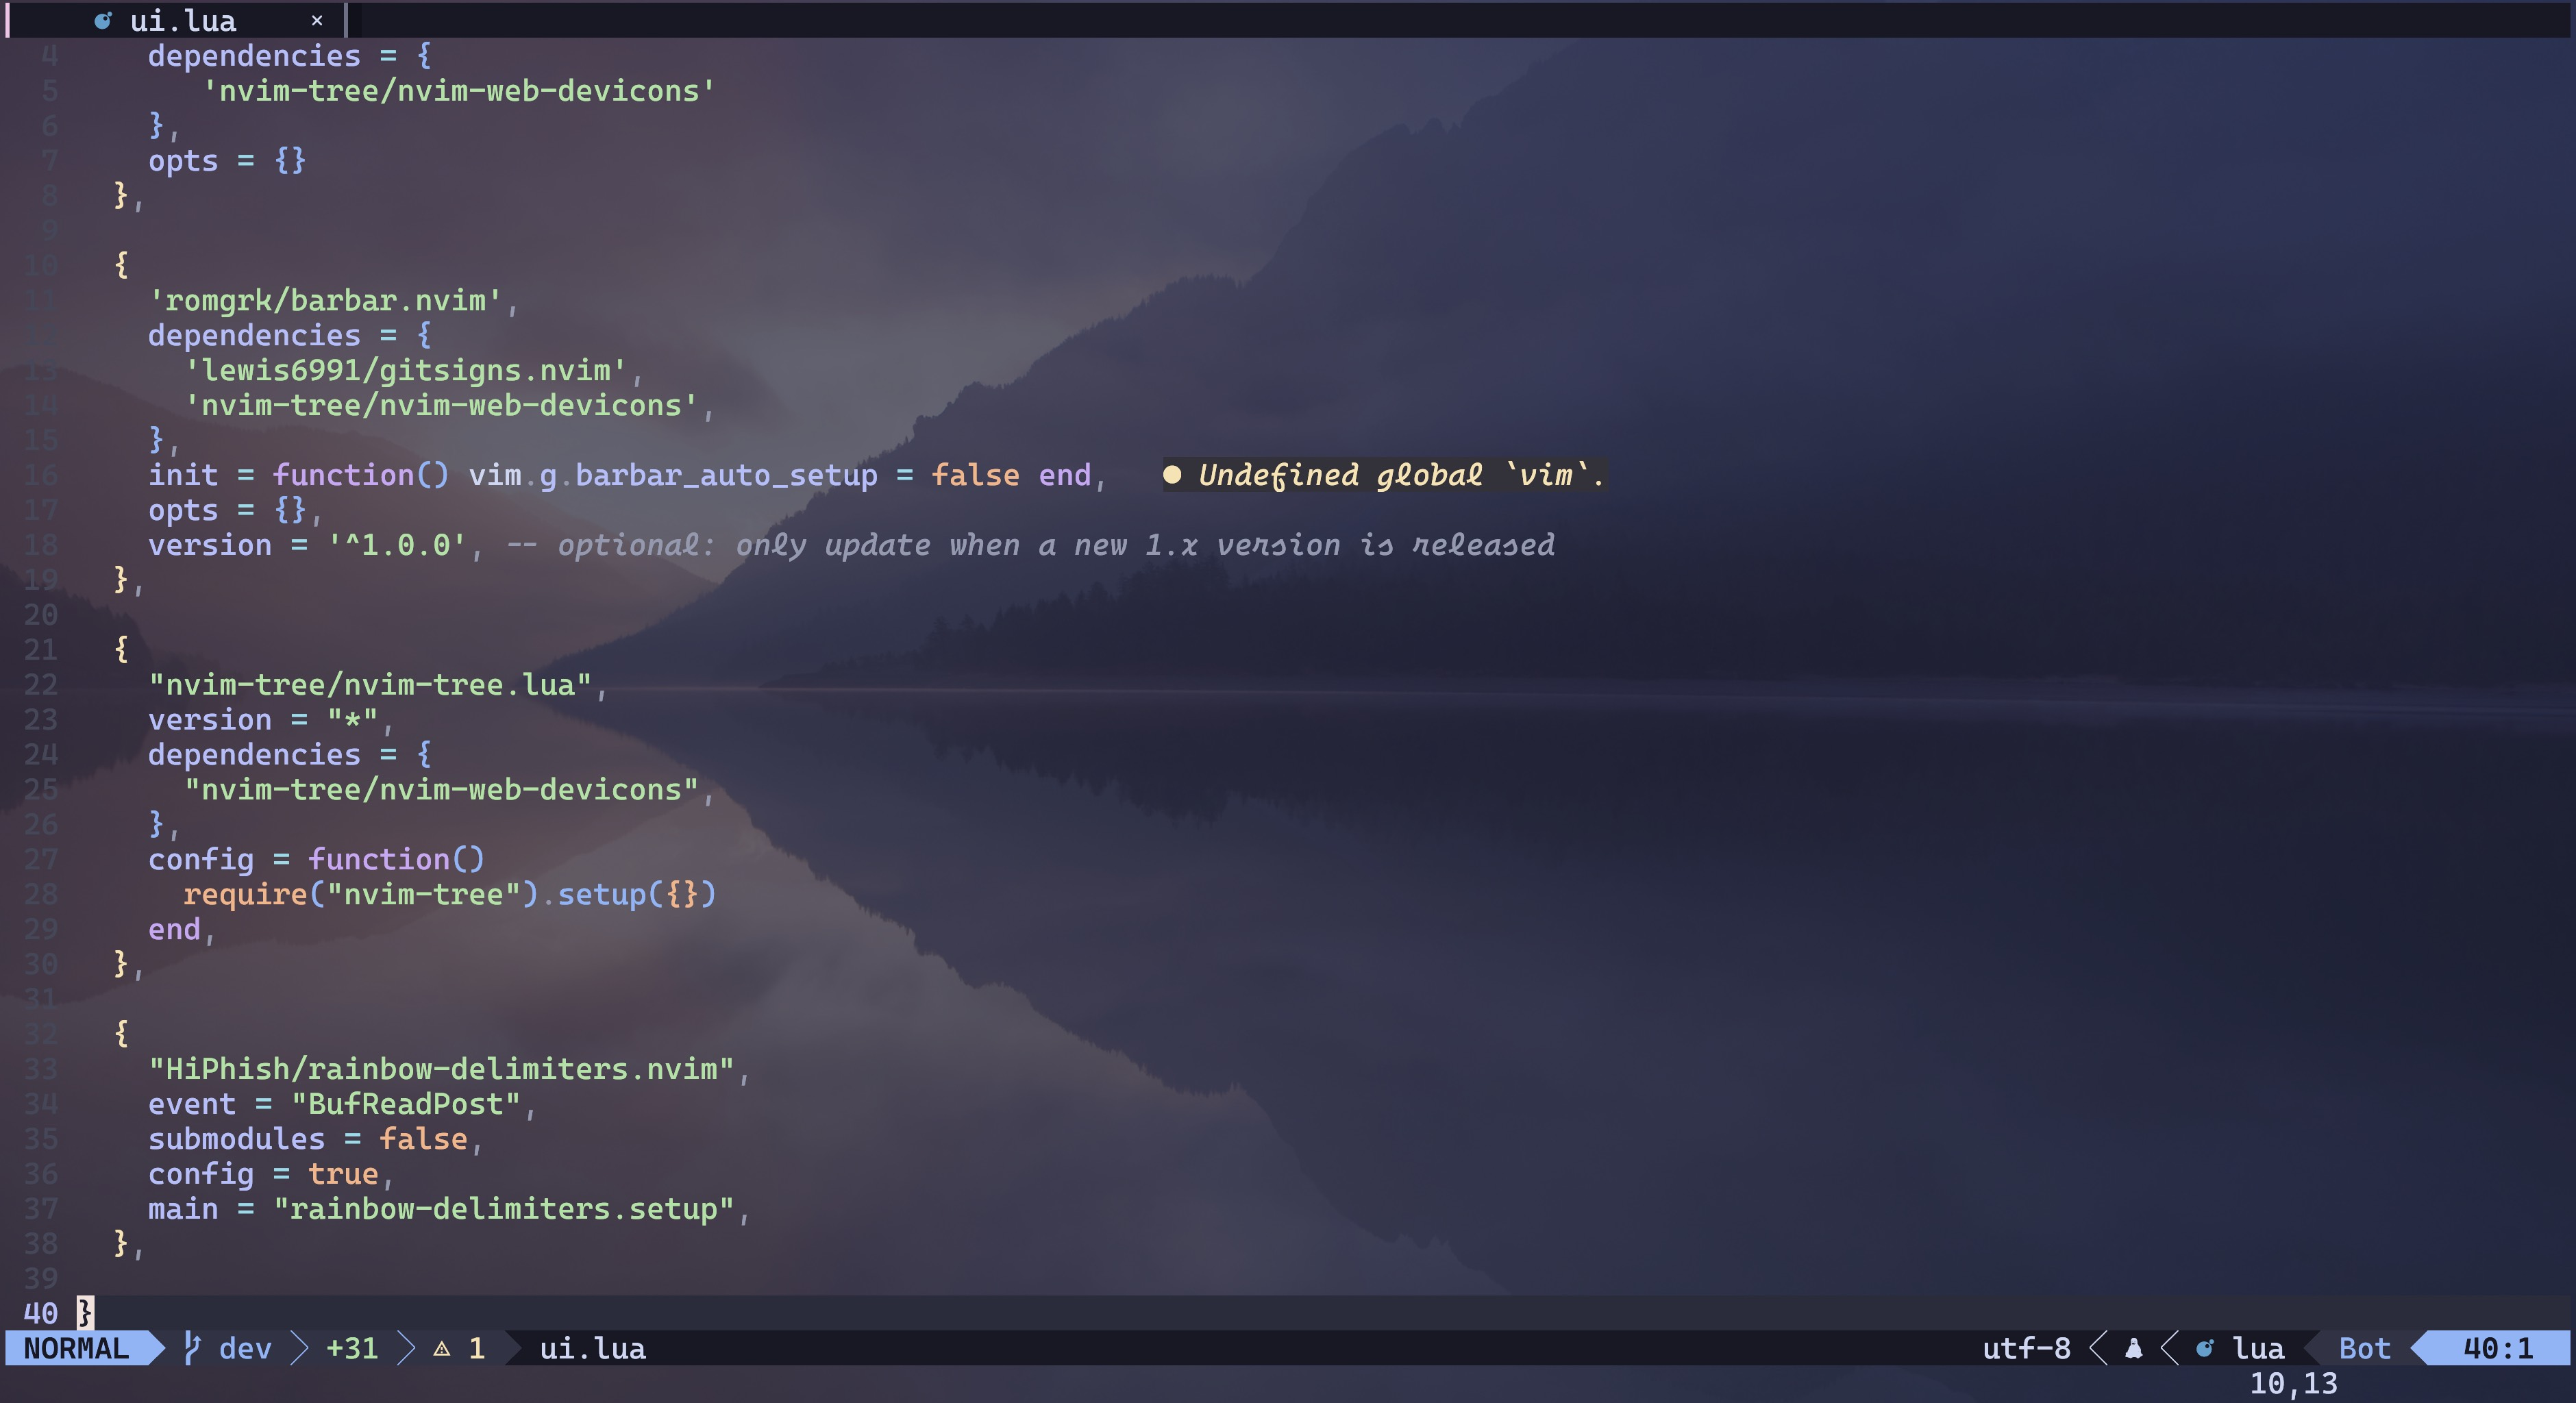
\includegraphics[width=\linewidth]{./Figures/Rainbow_Finish.jpg}
            \caption{安装后的效果}%
          \end{figure}

        \end{column}
      \end{columns}

    \end{frame}

  \subsection{UI美化:noice.nvim}

    \begin{frame}[fragile]{noice.nvim}

      \link{noice.nvim}{https://github.com/folke/noice.nvim}:更好看的消息界面和弹出式菜单 % ChkTeX 19

      \begin{columns}
        \begin{column}{0.4\linewidth}
          \begin{lstlisting}[basicstyle=\tiny\ttfamily]
-- ~/.config/nvim/lua/plugins/ui.lua

{
  "folke/noice.nvim",
  event = "VeryLazy",
  dependencies = {
    -- if you lazy-load any plugin below, make sure to add proper `module="..."` entries
    "MunifTanjim/nui.nvim",
    -- OPTIONAL:
    --   `nvim-notify` is only needed, if you want to use the notification view.
    --   If not available, we use `mini` as the fallback
    "rcarriga/nvim-notify",
  }
  opts = {},
}
          \end{lstlisting}
        \end{column}

        \begin{column}{0.6\linewidth}

          \begin{figure}[H]
            \centering
            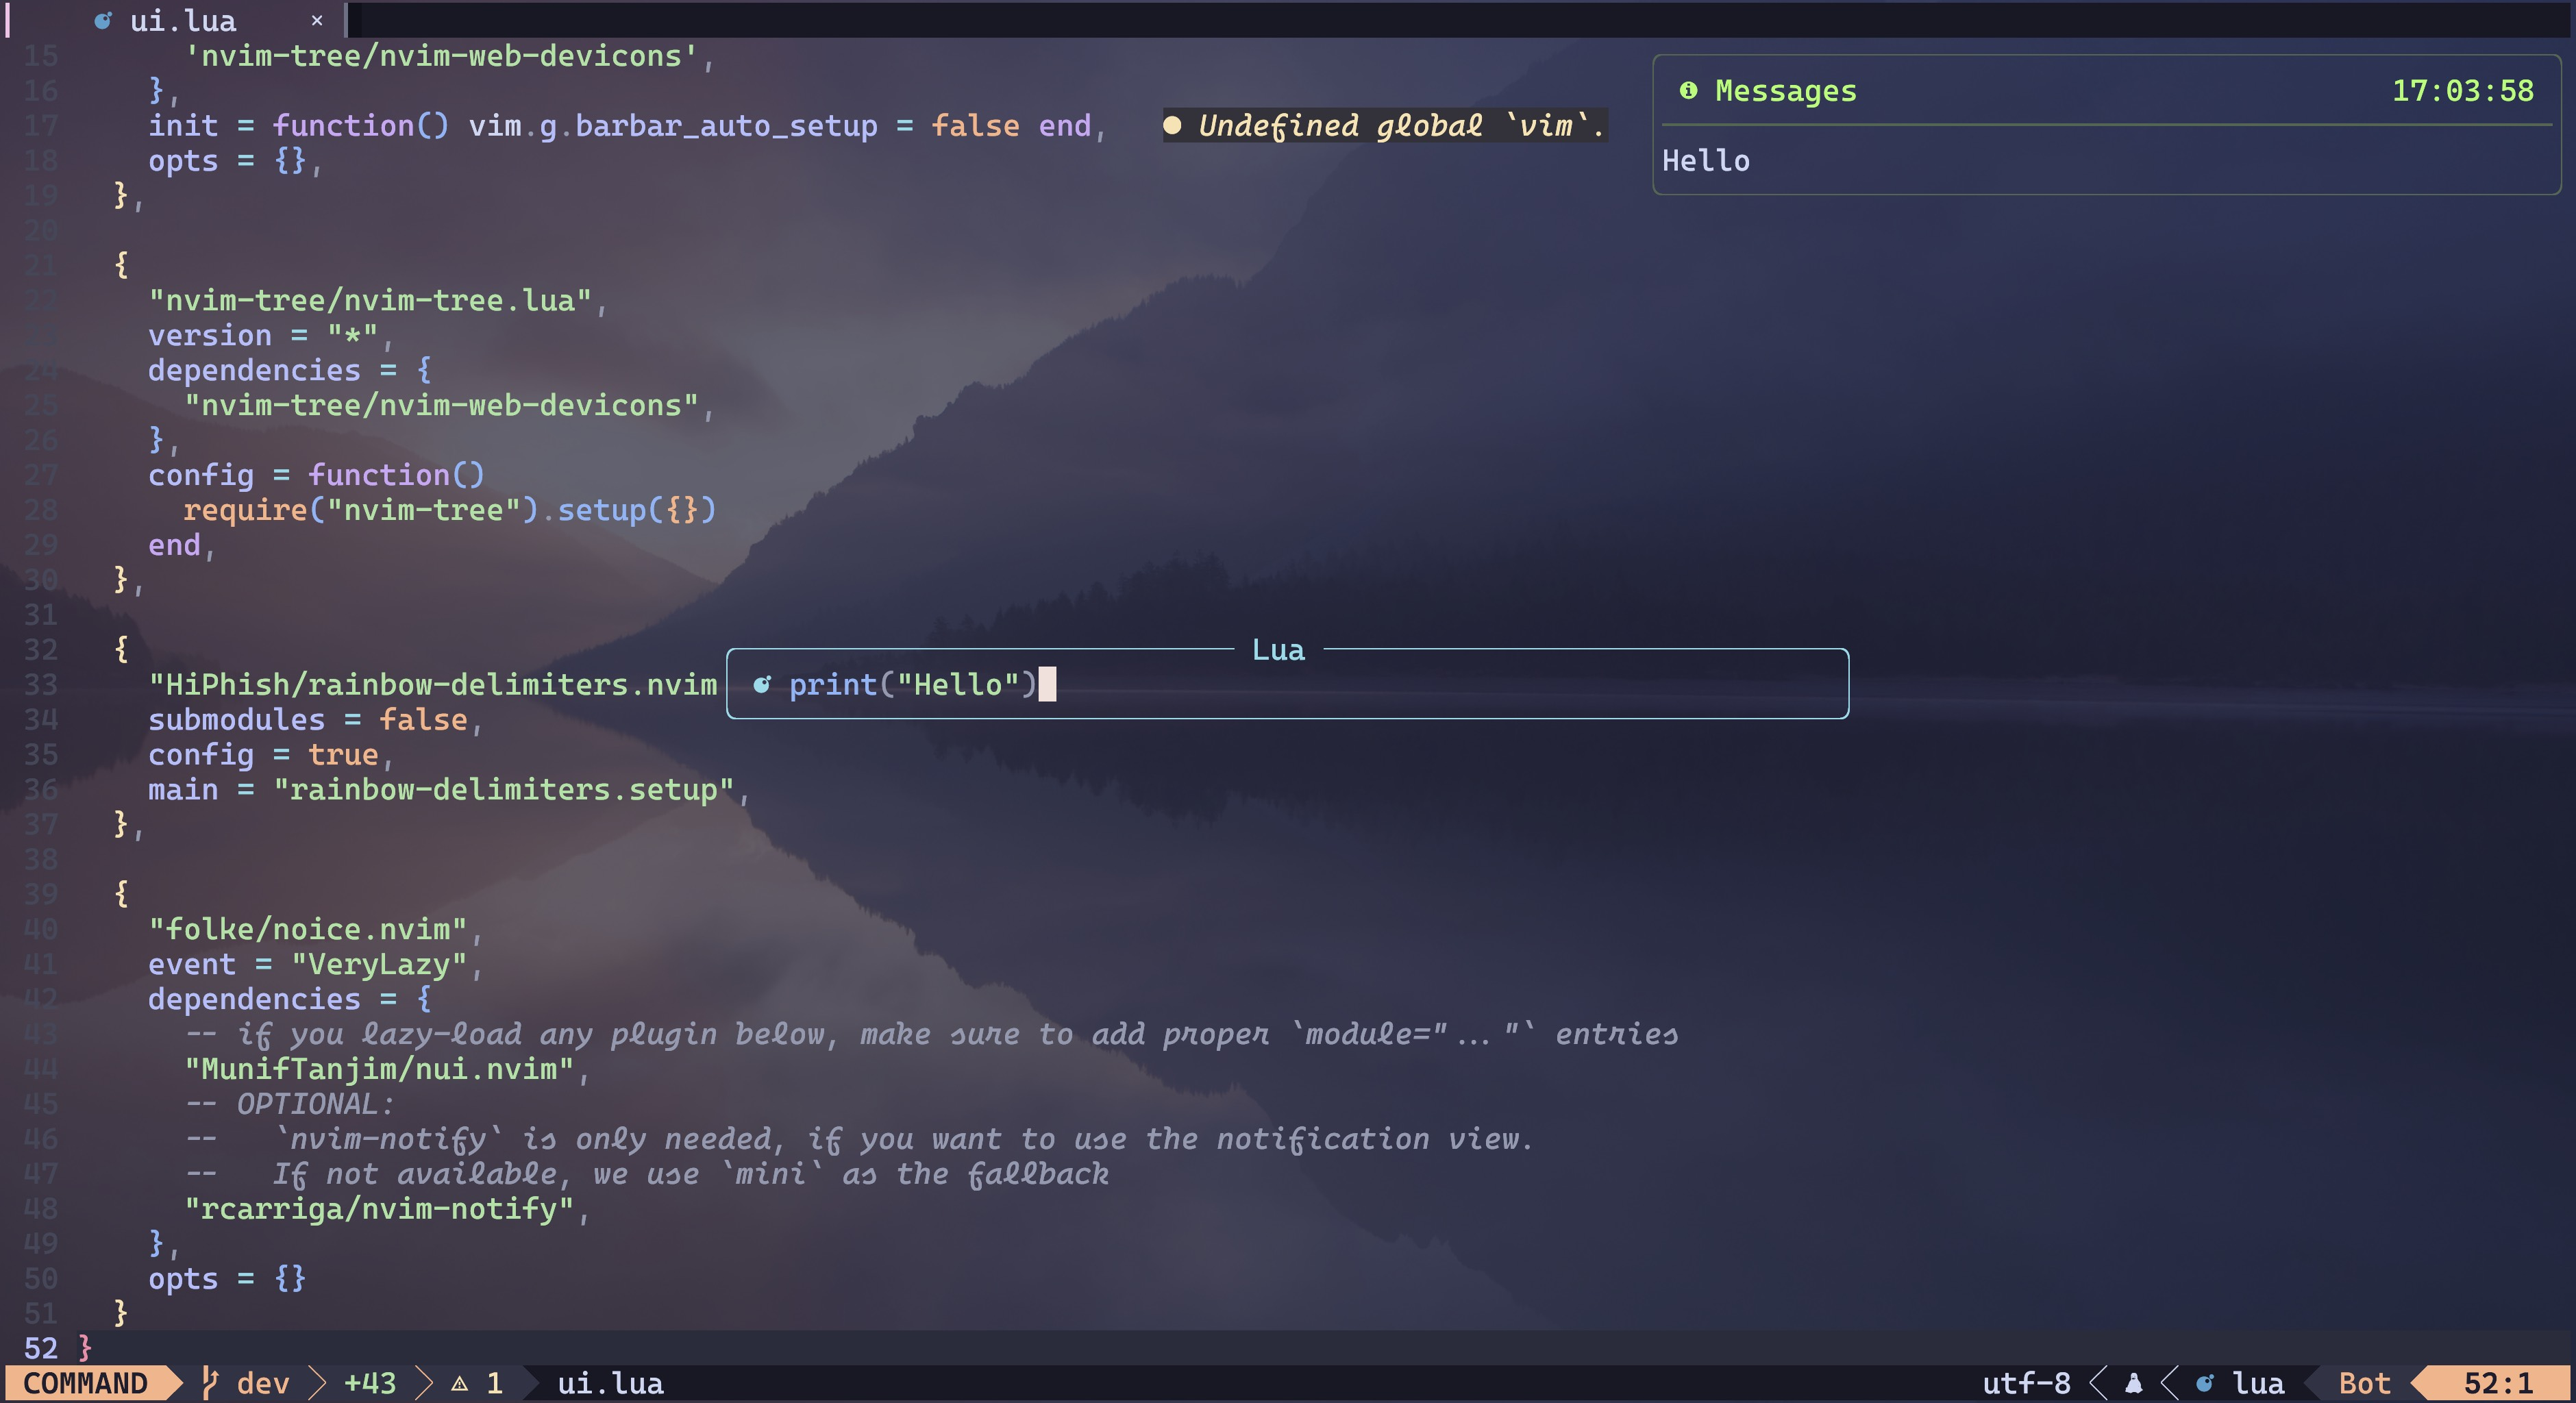
\includegraphics[width=\linewidth]{./Figures/Noice_Finish.jpg}
            \caption{安装后的效果}%
          \end{figure}

        \end{column}
      \end{columns}

    \end{frame}

\section{插件配置}

  \begin{frame}{插件配置}
    见演示

    \begin{itemize}
      \item catppuccin/nvim: \lstinline[language={},style=path]{\~/.config/nvim/lua/plugins/colorscheme.lua}
      \item Other plugins: \lstinline[language={},style=path]{\~/.config/nvim/lua/plugins/ui.lua}
    \end{itemize}
  \end{frame}

  \begin{frame}{最终效果}
    \begin{figure}[H]
      \centering
      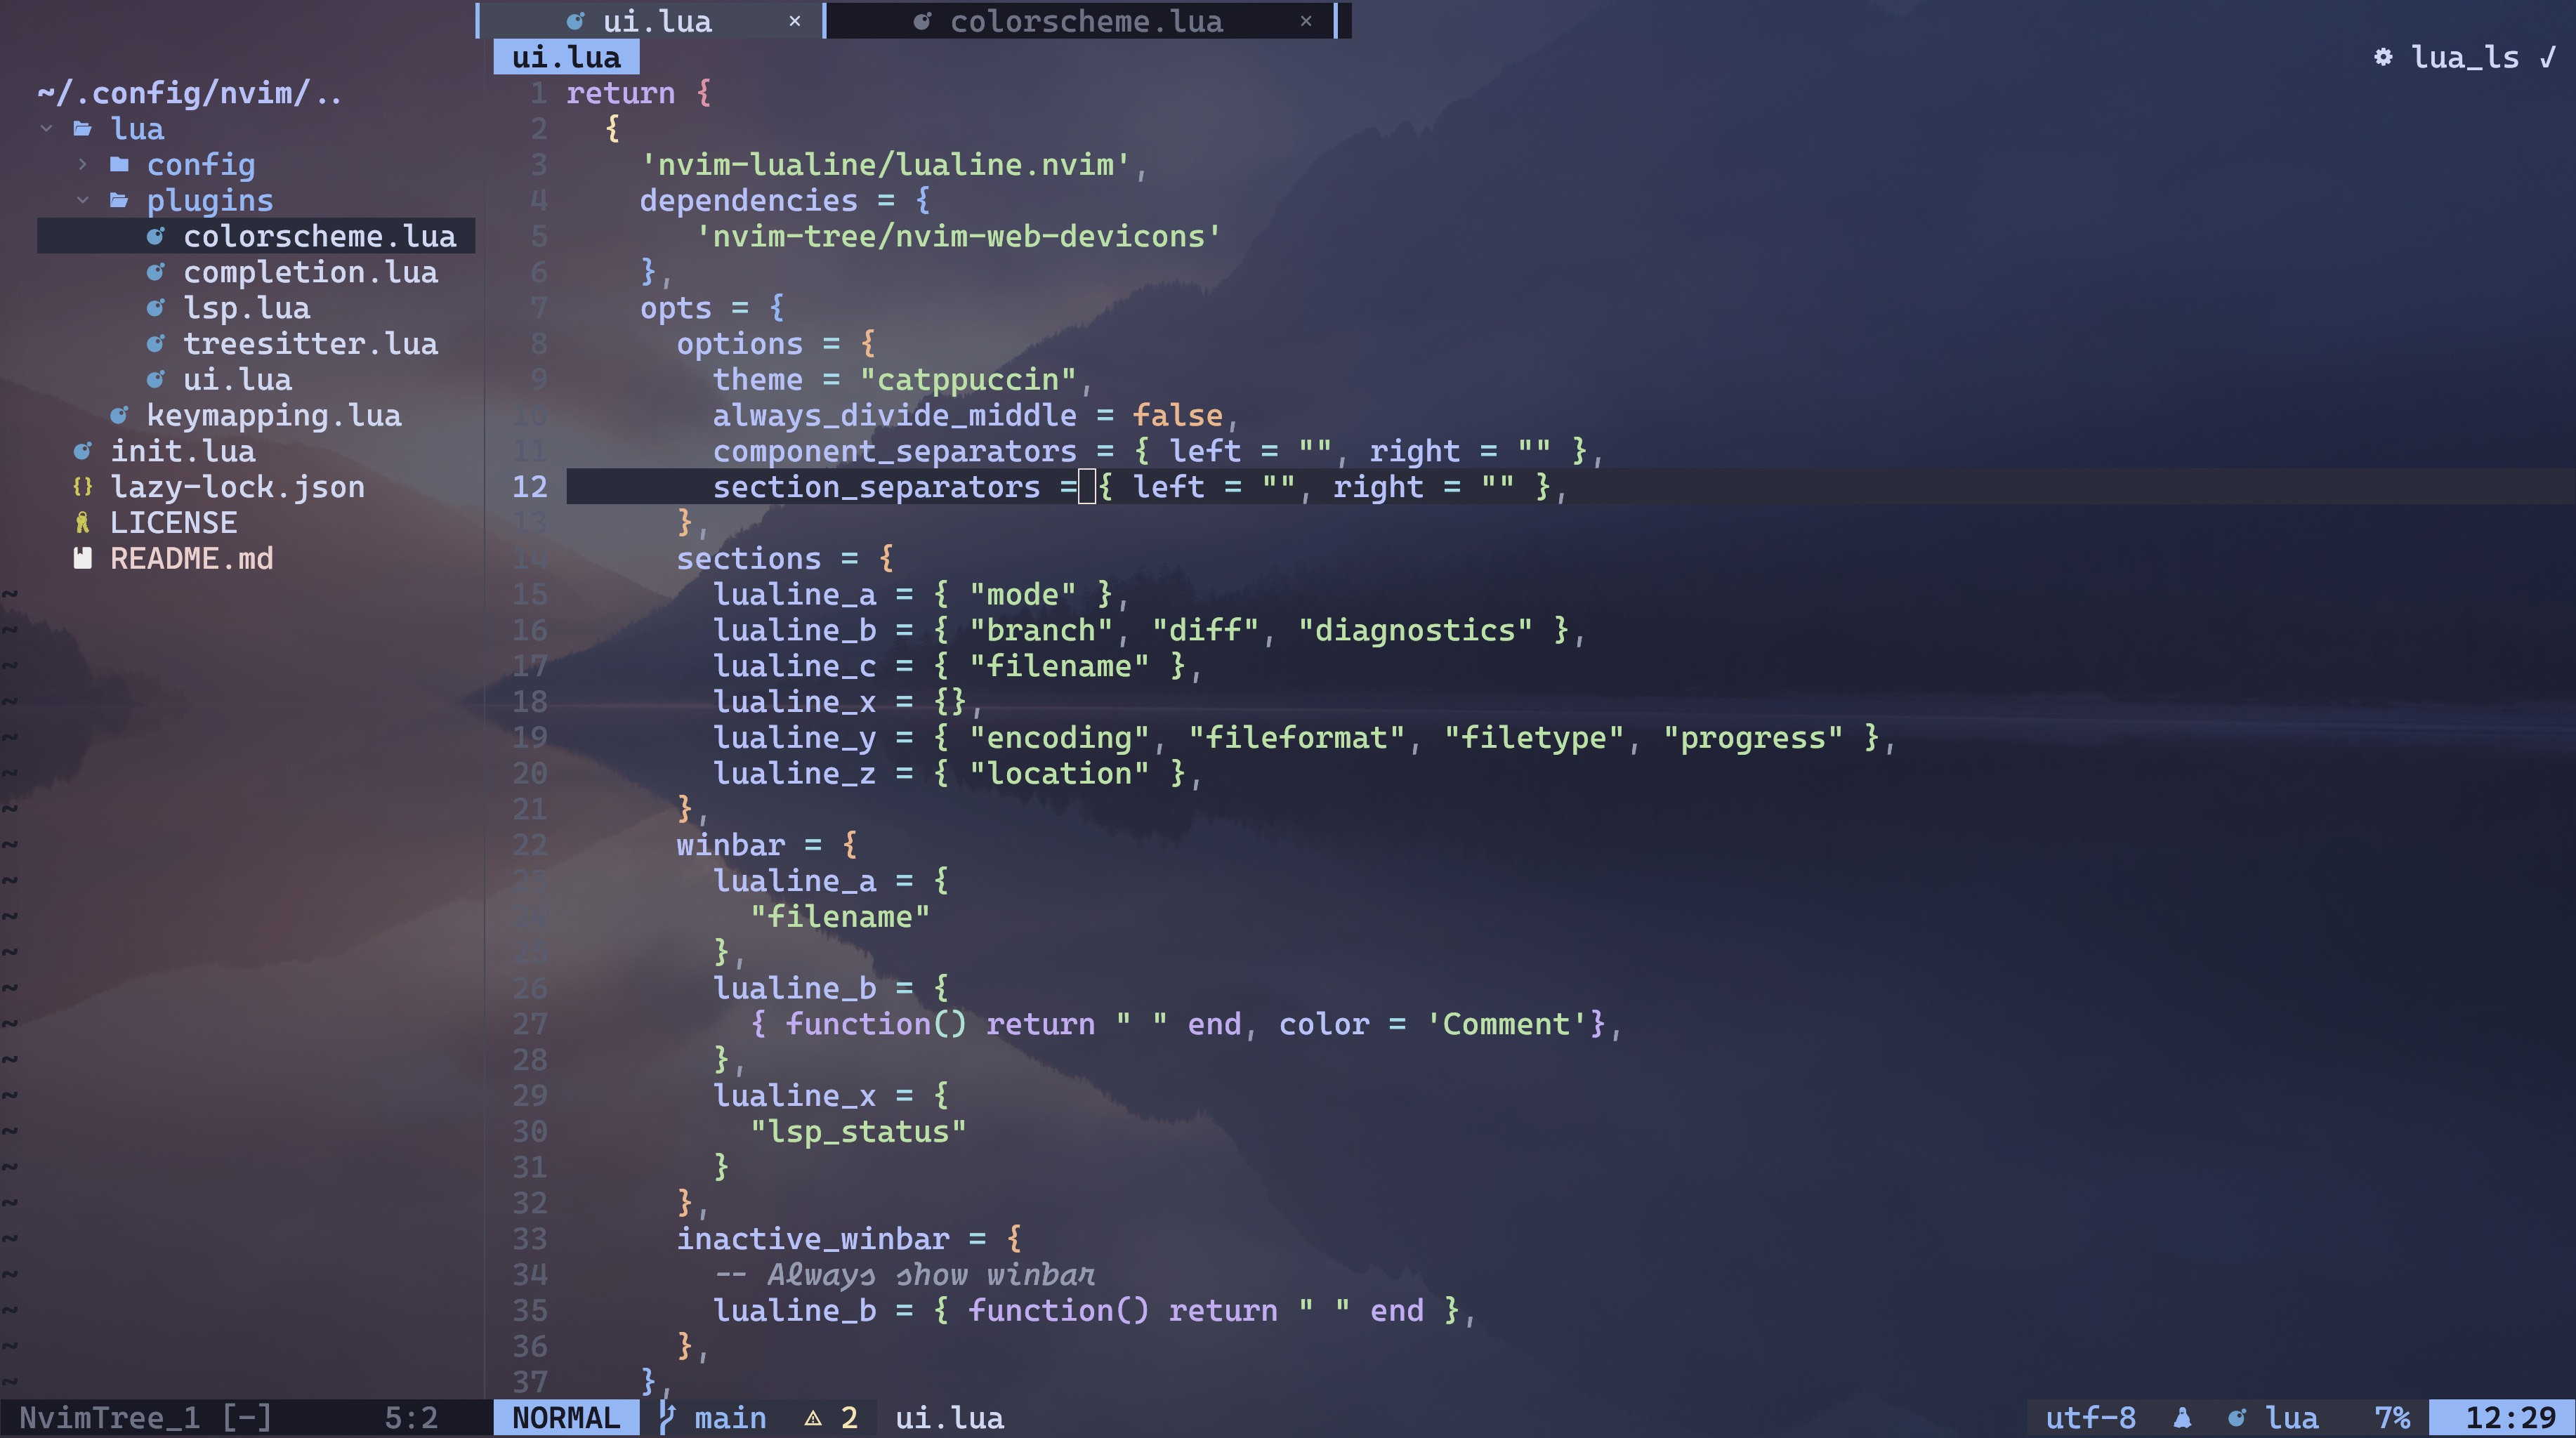
\includegraphics[width=0.75\linewidth]{./Figures/Final_Result.jpg}
    \end{figure}
  \end{frame}

  \begin{frame}
    \begin{itemize}
      \item 感谢:
        \begin{itemize}
          \item \link{Catppuccin}{https://catppuccin.com/} 
\includegraphics[height=10pt]{./Figures/Catppuccin_logo.png}
          \item \link{Catppuccin for beamer}{https://github.com/atticus-sullivan/beamercolortheme}
        \end{itemize}
        \vspace{0.5cm}
      \item 本教程的全部材料可以在我的Github上找到
        \begin{itemize}
          \item Slides: \url{https://github.com/Jacky-Lzx/nvim.tutorial.slides}
          \item Config: \url{https://github.com/Jacky-Lzx/nvim.tutorial.config}
        \end{itemize}
    \end{itemize}
  \end{frame}

\end{document}
